\documentclass[12pt,dvipdfmx]{book}
\usepackage{lmodern}
\usepackage[margin=1in]{geometry}
\usepackage{amsmath,amssymb,amsfonts,mathtools,amsthm}
\usepackage[dvipdfmx]{graphicx}
\usepackage{tcolorbox}
\usepackage{physics}
%\usepackage{slashbox}
%\usepackage{wrapfig}
%\usepackage{url,xspace,ascmac}
%\usepackage[]{xcolor}
%\usepackage{tcolorbox,todonotes}
\tcbuselibrary{breakable, skins, theorems}
%\usepackage{svg}
%\usepackage{etoolbox}
%\usepackage[subrefformat=parens]{subcaption}
%\usepackage{algorithm}
%\usepackage{algorithmic}
\usepackage[normalem]{ulem}
\usepackage{comment,tikz}
\usepackage{complexity}
\let\E\undefined
%\usepackage{todonotes}
%\usepackage{thmtools,thm-restate}
\usepackage{enumitem}
%\usepackage{ifthen}
%\usepackage{float}

\usetikzlibrary{positioning,calc}

\tikzset{every picture/.style={font issue=\footnotesize},
            font issue/.style={execute at begin picture={#1\selectfont}}
        }

\usepackage[unicode,colorlinks=true,citecolor=blue,linkcolor=blue,pdfusetitle]{hyperref}
\usepackage[style=alphabetic,natbib=true,natbib=true,maxnames=99,maxalphanames=99,isbn=false,url=false,backref=true,backend=biber,giveninits=true]{biblatex}

%\usepackage[style=alphabetic,natbib=true,maxnames=99,maxalphanames=99]{biblatex}
\addbibresource{ref.bib}

\usepackage{cleveref}

\newcommand{\crefpairconjunction}{と}
\newcommand{\crefrangeconjunction}{から}
\newcommand{\crefmiddleconjunction}{,}
\newcommand{\creflastconjunction}{,}

\newcommand{\kara}{} %無を出力するコマンド

%def
\newtcolorbox[auto counter, number within=section, crefname = {定義}{定義}]{definition}[3][]
{enhanced, breakable = true, fonttitle = \bfseries,
title = 定義~\thetcbcounter~\if #2\kara \else(#2) \fi,
#1,
label = def:#3}

%thm
\newtcolorbox[auto counter, use counter from=definition, crefname = {定理}{定理}]{theorem}[3][]
{enhanced, colback = orange!10!white, colframe = red!50!black, breakable = true, fonttitle = \bfseries,
title = 定理~\thetcbcounter~\if #2\kara \else(#2) \fi,
#1,
label = thm:#3}

%prop
\newtcolorbox[auto counter, use counter from=definition, crefname = {命題}{命題}]{proposition}[3][]
{enhanced,  colback = orange!10!white, colframe = red!50!black, breakable = true, fonttitle = \bfseries,
title = 命題~\thetcbcounter~\if #2\kara \else(#2) \fi,
#1,
label = prop:#3}

%lemma
\newtcolorbox[auto counter, use counter from=definition, crefname = {補題}{補題}]{lemma}[3][]
{enhanced,  colback = green!10!white, colframe = green!50!black, breakable = true, fonttitle = \bfseries,
title = 補題~\thetcbcounter~\if #2\kara \else(#2) \fi,
#1,
label = lem:#3}

%cor
\newtcolorbox[auto counter, use counter from=definition, crefname = {系}{系}]{corollary}[3][]
{enhanced, breakable = true, fonttitle = \bfseries,
title = 系~\thetcbcounter~\if #2\kara \else(#2) \fi,
#1,
label = cor:#3}

%remark
\newtcolorbox[auto counter, use counter from=definition, crefname = {注釈}{注釈}]{remark}[3][]
{enhanced, breakable = true, colback = white, fonttitle = \bfseries,
title = 注釈~\thetcbcounter~\if #2\kara \else(#2) \fi,
#1,
label = rem:#3}

%exercise
\newtcolorbox[auto counter, crefname = {演習問題}{演習問題}]{exercise}[3][]
{enhanced, breakable = true, colback = blue!10!white, colframe = blue!50!black, fonttitle = \bfseries,
title = 演習問題~\thetcbcounter~\if #2\kara \else(#2) \fi,
#1,
label = exer:#3}

%example
\newtcolorbox[auto counter, use counter from=definition, crefname = {例}{例}]{example}[3][]
{enhanced, breakable = true, colback = brown!10!white, colframe = brown!50!black, fonttitle = \bfseries,
title = 例~\thetcbcounter~\if #2\kara \else(#2) \fi,
#1,
label = ex:#3}

%algorithm
\newtcolorbox[auto counter, use counter from=definition, crefname = {アルゴリズム}{アルゴリズム}]{algorithm}[3][]
{enhanced, breakable = true, colback = cyan!10!white, colframe = cyan!50!black, fonttitle = \bfseries,
title = アルゴリズム~\thetcbcounter~\if #2\kara \else(#2) \fi,
#1,
label = alg:#3}

%claim
\newtcolorbox[auto counter, use counter from=definition, crefname = {主張}{主張}]{claim}[3][]
{enhanced, breakable = true, colback = yellow!10!white, colframe = yellow!50!black, fonttitle = \bfseries,
title = 主張~\thetcbcounter~\if #2\kara \else(#2) \fi,
#1,
label = claim:#3}

\renewcommand{\proofname}{\textbf{証明}}
\renewcommand{\figurename}{図}
\crefname{equation}{式}{式}
\crefname{section}{セクション}{セクション}
\crefname{figure}{図}{図}
\newcommand{\defeq}{\mathrel{:=}}
\DeclarePairedDelimiter{\floor}{\lfloor}{\rfloor} % floor function
\DeclarePairedDelimiter{\ceil}{\lceil}{\rceil} % ceil function
\let\ip\undefined
\DeclarePairedDelimiter{\ip}{\langle}{\rangle} % inner product

\newcommand{\Ver}{\mathrm{Ver}}
\newcommand{\Maj}{\mathrm{Maj}}
\newcommand{\indicator}[1]{\mathbf{1}_{#1}}
\newcommand{\condition}{\;\middle\vert\;}
\newcommand{\tand}{\text{ and }}
\newcommand{\tor}{\text{ or }}
\newcommand{\tif}{\text{if }}
\newcommand{\totherwise}{\text{otherwise}}

\newcommand{\Bin}{\mathrm{Bin}}

\newcommand{\true}{\mathsf{true}}
\newcommand{\false}{\mathsf{false}}
\newcommand{\e}{\mathrm{e}}
\DeclareMathOperator*{\E}{\mathbb{E}}
\DeclareMathOperator*{\Var}{\mathbf{Var}}
\newcommand{\dtv}{d_{\mathrm{TV}}}
\newcommand{\F}{\mathbb{F}}
\newcommand{\diam}{\mathrm{diam}}
\newcommand{\Fq}{\mathbb{F}_q}
\newcommand{\dist}{\mathrm{dist}}
\newcommand{\Nat}{\mathbb{N}}
\newcommand{\Real}{\mathbb{R}}
\newcommand{\Int}{\mathbb{Z}}
\newcommand{\Comp}{\mathbb{C}}
\newcommand{\binset}{\{0,1\}}
\newcommand{\supp}{\mathsf{supp}}
\renewcommand{\emph}[1]{\textbf{#1}}
\newcommand{\allone}{\mathbf{1}}
\newcommand{\Cay}{\mathrm{Cay}}

\newcommand{\argmax}{\mathop{\mathrm{argmax}}}
\newcommand{\RW}{\mathsf{RW}}

\newcommand{\val}{\mathrm{val}}
\newcommand{\UNSAT}{\mathrm{UNSAT}}
\renewcommand{\epsilon}{\varepsilon}
\newcommand{\size}{\mathrm{size}}

\newcommand{\PRIMES}{\mathrm{Primes}}
\newcommand{\ThreeCOL}{\mathrm{3COL}}
\newcommand{\LinEq}{\mathrm{LinEQ}}
\newcommand{\QuadEQ}{\mathrm{QuadEq}}
\newcommand{\ThreeQuadEQ}{\mathrm{3-QuadEq}}

\newcommand{\RS}{\mathrm{RS}}
\newcommand{\RM}{\mathrm{RM}}
\newcommand{\Had}{\mathrm{Had}}
\newcommand{\restr}[1]{|_{#1}}

\newcommand{\calA}{\mathcal{A}}
\newcommand{\calB}{\mathcal{B}}
\newcommand{\calC}{\mathcal{C}}
\newcommand{\calD}{\mathcal{D}}
\newcommand{\calE}{\mathcal{E}}
\newcommand{\calF}{\mathcal{F}}
\newcommand{\calG}{\mathcal{G}}
\newcommand{\calH}{\mathcal{H}}
\newcommand{\calI}{\mathcal{I}}
\newcommand{\calJ}{\mathcal{J}}
\newcommand{\calK}{\mathcal{K}}
\newcommand{\calL}{\mathcal{L}}
\newcommand{\calM}{\mathcal{M}}
\newcommand{\calN}{\mathcal{N}}
\newcommand{\calO}{\mathcal{O}}
\newcommand{\calP}{\mathcal{P}}
\newcommand{\calQ}{\mathcal{Q}}
\newcommand{\calR}{\mathcal{R}}
\newcommand{\calS}{\mathcal{S}}
\newcommand{\calT}{\mathcal{T}}
\newcommand{\calU}{\mathcal{U}}
\newcommand{\calV}{\mathcal{V}}
\newcommand{\calW}{\mathcal{W}}
\newcommand{\calX}{\mathcal{X}}
\newcommand{\calY}{\mathcal{Y}}
\newcommand{\calZ}{\mathcal{Z}}

\newcommand{\bolda}{\boldsymbol{a}}
\newcommand{\boldb}{\boldsymbol{b}}
\newcommand{\boldc}{\boldsymbol{c}}
\newcommand{\boldd}{\boldsymbol{d}}
\newcommand{\bolde}{\boldsymbol{e}}
\newcommand{\boldf}{\boldsymbol{f}}
\newcommand{\boldg}{\boldsymbol{g}}
\newcommand{\boldh}{\boldsymbol{h}}
\newcommand{\boldi}{\boldsymbol{i}}
\newcommand{\boldj}{\boldsymbol{j}}
\newcommand{\boldk}{\boldsymbol{k}}
\newcommand{\boldl}{\boldsymbol{l}}
\newcommand{\boldm}{\boldsymbol{m}}
\newcommand{\boldn}{\boldsymbol{n}}
\newcommand{\boldo}{\boldsymbol{o}}
\newcommand{\boldp}{\boldsymbol{p}}
\newcommand{\boldq}{\boldsymbol{q}}
\newcommand{\boldr}{\boldsymbol{r}}
\newcommand{\bolds}{\boldsymbol{s}}
\newcommand{\boldt}{\boldsymbol{t}}
\newcommand{\boldu}{\boldsymbol{u}}
\newcommand{\boldv}{\boldsymbol{v}}
\newcommand{\boldw}{\boldsymbol{w}}
\newcommand{\boldx}{\boldsymbol{x}}
\newcommand{\boldy}{\boldsymbol{y}}
\newcommand{\boldz}{\boldsymbol{z}}

\newcommand{\boldA}{\boldsymbol{A}}
\newcommand{\boldB}{\boldsymbol{B}}
\newcommand{\boldC}{\boldsymbol{C}}
\newcommand{\boldD}{\boldsymbol{D}}
\newcommand{\boldE}{\boldsymbol{E}}
\newcommand{\boldF}{\boldsymbol{F}}
\newcommand{\boldG}{\boldsymbol{G}}
\newcommand{\boldH}{\boldsymbol{H}}
\newcommand{\boldI}{\boldsymbol{I}}
\newcommand{\boldJ}{\boldsymbol{J}}
\newcommand{\boldK}{\boldsymbol{K}}
\newcommand{\boldL}{\boldsymbol{L}}
\newcommand{\boldM}{\boldsymbol{M}}
\newcommand{\boldN}{\boldsymbol{N}}
\newcommand{\boldO}{\boldsymbol{O}}
\newcommand{\boldP}{\boldsymbol{P}}
\newcommand{\boldQ}{\boldsymbol{Q}}
\newcommand{\boldR}{\boldsymbol{R}}
\newcommand{\boldS}{\boldsymbol{S}}
\newcommand{\boldT}{\boldsymbol{T}}
\newcommand{\boldU}{\boldsymbol{U}}
\newcommand{\boldV}{\boldsymbol{V}}
\newcommand{\boldW}{\boldsymbol{W}}
\newcommand{\boldX}{\boldsymbol{X}}
\newcommand{\boldY}{\boldsymbol{Y}}
\newcommand{\boldZ}{\boldsymbol{Z}}

\newcommand{\veca}{\vec{a}}
\newcommand{\vecb}{\vec{b}}
\newcommand{\vecc}{\vec{c}}
\newcommand{\vecd}{\vec{d}}
\newcommand{\vece}{\vec{e}}
\newcommand{\vecf}{\vec{f}}
\newcommand{\vecg}{\vec{g}}
\newcommand{\vech}{\vec{h}}
\newcommand{\veci}{\vec{i}}
\newcommand{\vecj}{\vec{j}}
\newcommand{\veck}{\vec{k}}
\newcommand{\vecl}{\vec{l}}
\newcommand{\vecm}{\vec{m}}
\newcommand{\vecn}{\vec{n}}
\newcommand{\veco}{\vec{o}}
\newcommand{\vecp}{\vec{p}}
\newcommand{\vecq}{\vec{q}}
\newcommand{\vecr}{\vec{r}}
\newcommand{\vecs}{\vec{s}}
\newcommand{\vect}{\vec{t}}
\newcommand{\vecu}{\vec{u}}
\newcommand{\vecv}{\vec{v}}
\newcommand{\vecw}{\vec{w}}
\newcommand{\vecx}{\vec{x}}
\newcommand{\vecy}{\vec{y}}
\newcommand{\vecz}{\vec{z}}

\newcommand{\bara}{\overline{a}}
\newcommand{\barb}{\overline{b}}
\newcommand{\barc}{\overline{c}}
\newcommand{\bard}{\overline{d}}
\newcommand{\bare}{\overline{e}}
\newcommand{\barf}{\overline{f}}
\newcommand{\barg}{\overline{g}}
\newcommand{\barh}{\overline{h}}
\newcommand{\bari}{\overline{i}}
\newcommand{\barj}{\overline{j}}
\newcommand{\bark}{\overline{k}}
\newcommand{\barl}{\overline{l}}
\newcommand{\barm}{\overline{m}}
\newcommand{\barn}{\overline{n}}
\newcommand{\baro}{\overline{o}}
\newcommand{\barp}{\overline{p}}
\newcommand{\barq}{\overline{q}}
\newcommand{\barr}{\overline{r}}
\newcommand{\bars}{\overline{s}}
\newcommand{\bart}{\overline{t}}
\newcommand{\baru}{\overline{u}}
\newcommand{\barv}{\overline{v}}
\newcommand{\barw}{\overline{w}}
\newcommand{\barx}{\overline{x}}
\newcommand{\bary}{\overline{y}}
\newcommand{\barz}{\overline{z}}

\newcommand{\boldalpha}{\boldsymbol{\alpha}}
\newcommand{\boldbeta}{\boldsymbol{\beta}}
\newcommand{\boldgamma}{\boldsymbol{\gamma}}
\newcommand{\bolddelta}{\boldsymbol{\delta}}
\newcommand{\boldepsilon}{\boldsymbol{\epsilon}}
\newcommand{\boldzeta}{\boldsymbol{\zeta}}
\newcommand{\boldeta}{\boldsymbol{\eta}}
\newcommand{\boldtheta}{\boldsymbol{\theta}}
\newcommand{\boldiota}{\boldsymbol{\iota}}
\newcommand{\boldkappa}{\boldsymbol{\kappa}}
\newcommand{\boldlambda}{\boldsymbol{\lambda}}
\newcommand{\boldmu}{\boldsymbol{\mu}}
\newcommand{\boldnu}{\boldsymbol{\nu}}
\newcommand{\boldxi}{\boldsymbol{\xi}}
\newcommand{\boldpi}{\boldsymbol{\pi}}
\newcommand{\boldrho}{\boldsymbol{\rho}}
\newcommand{\boldsigma}{\boldsymbol{\sigma}}
\newcommand{\boldtau}{\boldsymbol{\tau}}
\newcommand{\boldupsilon}{\boldsymbol{\upsilon}}
\newcommand{\boldphi}{\boldsymbol{\phi}}
\newcommand{\boldchi}{\boldsymbol{\chi}}
\newcommand{\boldpsi}{\boldsymbol{\psi}}
\newcommand{\boldomega}{\boldsymbol{\omega}}
\newcommand{\boldvarepsilon}{\boldsymbol{\varepsilon}}
\newcommand{\boldvartheta}{\boldsymbol{\vartheta}}
\newcommand{\boldvarrho}{\boldsymbol{\varrho}}
\newcommand{\boldvarsigma}{\boldsymbol{\varsigma}}
\newcommand{\boldvarphi}{\boldsymbol{\varphi}}
\newcommand{\boldvarpi}{\boldsymbol{\varpi}}

\newcommand{\varx}{\mathrm{x}}
\newcommand{\vary}{\mathrm{y}}

\title{PCP定理の証明と応用}
\author{清水 伸高 (東京科学大学)}
\date{}
\begin{document}
\maketitle
\tableofcontents
\chapter*{序文}



このノートは, 京都大学大学院理学研究科数学・数理解析専攻数理解析系で開催される集中講義「PCP定理の証明と応用」の講義ノートである.
計算量(computational complexity)とは, 問題を解くために必要な計算リソースの量(例えば計算時間, 記憶領域のサイズ, 乱択や量子性の有無や量)を意味し, 計算量理論(computational complexity theory)とはそれぞれの問題の計算量を明らかにするための理論である.
PCP定理とは, 判定問題(YesかNoで答える問題)の検証に要する計算量に関する結果であり,
端的に言うと, ある命題が真であると主張する証明が文字列として与えられたとき,
その証明を検証するためには, 通常, 全ての文字を見て確認する必要があるが,
PCP定理によれば, その証明の一部だけを見ることで, その命題が真であるか否かを確率的に検証することができるという驚くべき結果である.
例えば, ある実行列$A$と実ベクトル$b$に対して線形方程式系$Ax=b$は解を持つ, という命題を考えてみよう.
この命題が真であるならば実際に解の一つ$x$を証明として提示することができるが, その証明が正しいかどうかを検証するためには検証者は$Ax$を実際に計算し, その各成分が$b$と一致するかを確認する必要がある.
ところがPCP定理によれば, 巧妙に構成された証明$\pi$を提示することにより, その証明$\pi$全ての文字を見ることなく, 99\%の確率で正しく検証できるのである (ここでは確率的な検証, つまり検証者はランダムネスを用いた検証を行う設定を考える).

このように, 局所的な情報だけを使って全体の構造を推測できるというPCP定理の性質は, 単に理論的に興味深いだけでなく, 誤り訂正符号の構成, 確率論的手法の脱乱択化, 最適化問題の近似率限界の導出など, 理論計算機科学において広大な応用を持ち, 現在でも計算量理論の中心的な研究対象の一つである.
このような重要性を持つにもかかわらず, PCP定理の証明に包括的に日本語でアクセスできる文献は(筆者が知る限り本資料の執筆時点では)存在しない.
本講義ではPCP定理の証明を与えるとともに, その証明に用いられた計算量理論の基本的な概念や技法を解説し,
PCP定理の応用についても触れる.
僭越ながらもこれはPCP定理の証明に日本語でアクセスする(おそらく国内初の)資料であるといえる.
今回のような挑戦的な機会を与えてくださった河村彰星先生に感謝を申し上げる.

\addcontentsline{toc}{chapter}{Preface}
\chapter{導入}

この集中講義ではPCP定理と呼ばれる計算量理論の基本的な結果について解説し, その証明を与える.
PCP定理は1998年に\citet{AroraS98,AroraLMSS98}によって証明された.
この証明は代数的な手法に基づく誤り訂正符号を技巧的に組合せたものであり, 難解なものであったが, その後\citet{Din07}によってより簡潔な証明が与えられた.
この講義では\citet{Din07}による比較的簡単な証明を紹介する.
ちなみにDinurはのちにこの業績によりゲーデル賞を受賞している.

\section{検証能力}
\subsection{クラスNP}
\subsection{クラスAM}
\subsection{クラスPCP}

\section{PCP定理}

\subsection{自明な例}

\begin{theorem}{PCP定理}{PCPtheorem}
  ...
\end{theorem}


\section{制約充足問題(CSP)}
\subsection{充足可能性判定問題(SAT)}
\chapter{局所的な検証と弱いPCP定理の証明}

この章はPCP検証者における「少ないクエリ回数」という要件がなぜ達成できるかについて説明することを目的とする.
そのため, まずはPCP定理の要件であるランダムビットの短さはひとまず無視した以下の形の「弱いPCP定理」を証明する: 任意の$\NP$に属する判定問題が$O(1)$クエリかつ$\poly(n)$ビットのランダムネスを用いて確率的に検証可能である.

\section{局所的な検証}
本講義では, 検証者が証明の文字列$\pi$のうち$O(1)$個の文字を読み込んで検証を行うことを\emph{局所的な検証}と呼ぶことにする.
一般的な感覚として, ある主張が成り立つことを示す証明を検証する際, \emph{冗長に表現で記述しない限り}その証明を全て読み込まなければ検証できないと思われる (全ての文字に本質的な意味があるならば全てを確認しなければならないはずであろう).
では逆に, 証明を冗長に表現することで局所的な検証を可能にすることはできるだろうか?

\subsection{線形方程式の局所的な検証(1/2)}
興味深いことに, 非常に冗長性が大きい記述で証明が与えられたならば局所検証が可能であることを, 線形方程式の検証を例に説明する.

\begin{definition}{線形方程式}{linear-equation}
有限体$\F$上の行列$M\in\F^{m\times n}$とベクトル$z\in\F^m$に対して
\begin{align*}
  My = z
\end{align*}
を満たす$y\in\F^n$が存在するかどうかを判定する問題を$\LinEq$とする.
ここで$\abs{\F}=q$は$m,n$とは独立な定数であるとする (従って有限体上の演算は$O(1)$時間で計算できると仮定する).
\end{definition}

愚直な検証者として$y\in\F^n$を証拠として受け取り, $My=z$を確認することで検証を行うことを考える (実際の計算機では全てを二進文字列で表現するため, $\F$の元は$\ceil{\log_2\abs{\F}}=O(1)$ビットで表現されている).
明らかにこの検証者は$My$を計算するために$y$の全ての成分 (すなわち$O(n)$ビット) を読み込む必要があるため, 局所的な検証者とはならない.
もちろん, この判定問題は標準的な線型方程式の解の存在性判定であるため, 掃き出し法を用いれば証拠へのオラクルアクセスなしでも多項式時間で解ける.
しかしここではあえて, 局所的な検証の構成例を与えるという目的で取り扱う.

重要な性質として, 二つのベクトル$a,b\in\F^n$に対する次の性質を考える (証明は\cref{exer:random-inner-product}):
\begin{align}
  \Pr_{r\sim \F^n} \qty[ r^\top a \ne r^\top b ] = \begin{cases}
    0 & \text{if } a=b \\
    1-\frac{1}{q} & \text{if } a\ne b.
  \end{cases} \label{eq:linear-equation-property}
\end{align}
さて, \cref{eq:linear-equation-property}の性質を用いると一様ランダムな$r\sim\F^n$に対して
\begin{align}
  r^\top M y = r^\top z \label{eq:random-inner-product}
\end{align}
かどうかを確認することで, $My=z$かどうかを確率的に検証できる.
実際, $My=z$ならば確率$1$で検証者は受理し,
$My\ne z$ならば確率$1-1/q$で検証者は拒否する (何度も繰り返せばこの拒否率を任意に$1$に近い定数まで近づけることができる).
ベクトル$z$は入力として与えられているため\cref{eq:random-inner-product}の右辺は$O(n)$時間で計算できる.
一方で, ベクトル$y$は証拠として与えられるため, $r^\top M y$の計算は愚直に考えると$O(mn)$時間かかる上に$y$の全ての成分を読み込む必要がある.
ところが, 全てのベクトル$w\in \F^n$に対して$y^\top w\in\F$を連結して得られる長さ$q^n$の文字列$(y^\top w)_{w\in \F^n}$を証拠$\pi$として与えることにより,
自身で$r^\top M$を計算した後に $r^\top M y = y^\top (M^\top r)$の値を\emph{一文字の証拠の読み込み}で計算できるのである.

\begin{exercise}{ランダムなベクトルとの内積}{random-inner-product}
  \cref{eq:linear-equation-property}を証明せよ.
\end{exercise}

このように, ベクトル$y\in\F^n$を, それを係数とする線形関数$w\mapsto y^\top w$の\emph{真理値表(全ての点での評価値を並べた文字列)として冗長に表現する}ことで, 証拠の読み込み回数を定数に抑えるというのが基本的なアイデアである.
このように文字列を冗長に表現する手法を総称して\emph{誤り訂正符号}という.
本講義では, \emph{アダマール符号}と呼ばれる以下の誤り訂正符号を用いる:
\begin{definition}{アダマール符号}{Hadamard-code}
  有限体$\F$上のベクトル$y\in\F^n$に対して, 長さ$q^n$の文字列
  \begin{align*}
    \Had_n(y) = (y^\top w)_{w\in \F^n}
  \end{align*}
  を考える.
  集合$\Had_n = \qty{ \Had_n(y) \colon y\in \F^n }$を\emph{アダマール符号}といい,
  その元を\emph{アダマール符号の符号語}という.
  また, $\Had_n(y)$を\emph{$y$をアダマール符号で符号化した文字列}という.

  なお, 次元$n$が明らかなときは省略して$\Had(y)$などと表す.
\end{definition}

\begin{remark}{}{string-vector-function}
  本講義では文字列, ベクトル, 関数をしばし同一視する.
  すなわち, ベクトル$x\in\F^n$を単に文字列と呼ぶこともあり,
  または関数$x\colon [n]\to\F$とみなすこともある.
  例えば$y\in\F^n$をアダマール符号で符号化した文字列$\Had(y)$は, 長さ$q^n$の文字列とみなすこともあれば,
  関数$\Had(y)\colon \F^n\to\F$とみなすこともある.

  これは, アダマール符号の解析の過程では$\Had(y)$を関数とみなして扱う方が都合が良いものの,
  PCP定理の証明の過程では$\Had(y)$を文字列として扱い, 証明$\pi$として与えることになるからである.
\end{remark}

素朴な証拠$y$をアダマール符号で符号化したものを証明として扱うというアイデアを素朴に実装すると, $\LinEq$に対する局所的な検証(の候補)として以下の検証者を考えることができる:
\begin{algorithm}{$\LinEq$に対する局所的な検証?}{local-verification-LinEq?}
  \begin{enumerate}
  \item 入力として$M,z$を受け取り, 証拠として$\pi \in \F^{q^n}$へのオラクルアクセスを受け取る.
  \item 一様ランダムな$r\sim\F^m$を選択し, $r^\top M$と$r^\top z$を計算する.
  \item 証拠$\pi\colon \F^{q^n}$を関数$\pi\colon \F^n\to \F$として解釈し, オラクルアクセスを用いて$a=\pi(M^\top r)$を求める.
  \item $a=r^\top z$ならば$1$を出力し, そうでなければ$0$を出力する.
  \end{enumerate}
\end{algorithm}

上記の検証者はPCP検証者の性質を持つだろうか?
まず, $(M,z)$がYesインスタンスであるとき, ある$y\in\F^n$が存在して$My=z$が成り立つ.
このとき, $\pi=\Had(y)\colon\F^n\to\F$とすると, $\pi(M^\top r)=y^\top (M^\top r)=r^\top (My)=r^\top z$となるため, 検証者は確率$1$で受理する.

一方で$(M,z)$がNoインスタンスであるときに検証者が拒否する確率はどうなるだろうか?
PCP検証者であることを示す(cf. \cref{def:PCP})には, 任意の$\pi\in\F^n\to\F$に対して拒否確率は少なくとも$1/3$以上でなければならない.
これは示せるのであろうか?
証明$\pi$がアダマール符号の符号語である(すなわち, ある$y\in\F^n$に対して$\pi = \Had(y)$と表せる)場合は, \cref{eq:random-inner-product}の性質および$(M,z)$がNoインスタンスであることから$My\ne z$より, 少なくとも確率$1-1/q$で検証者は拒否する.
しかしながら, 一般の$\pi\in\F^n\to\F$はこのような線形関数として表現できるとは限らず, そのような$\pi$に対しても拒否しなければならない.

\subsection{線形性テスト}
与えられた$(M,z)$がNoインスタンスであるときに任意の$\pi\in\F^{q^n}$を定数確率で拒否するために,
\cref{alg:local-verification-LinEq?}を以下のように修正する:
証拠$\pi$がアダマール符号の符号語ならば, \cref{alg:local-verification-LinEq?}のステップ2-4を実行し, そうでないならば$0$を出力する.
ここで新たに一つの問題が生じる: どのようにして$\pi$の線形性を局所検証すればよいだろうか?

一般にオラクルアクセスで与えられた関数$\pi\colon\F^n\to\F$が線形関数かどうかを厳密に確認するには,
\begin{align}
  \forall x,y\in\F^n,\quad \pi(x+y)=\pi(x)+\pi(y) \label{eq:linearity-test-all-points}
\end{align}
が成り立つかどうかを確認する必要があり, $q^n$回のオラクルアクセスが必要となってしまう.

そこで, 「線形関数であるかどうか」ではなく「線形関数に近いかどうか」を局所検証することを考える.
\begin{definition}{関数同士の近さ}{distance-between-functions}
  二つの関数$f,g\colon A \to B$に対して$\dist(f,g)$を
  \begin{align*}
    \dist(f,g) =\Pr_{a\sim A} \qty[ f(a) \ne g(a) ]
  \end{align*}
  と定義し, $\dist(f,g)\le\delta$を満たすとき, $f$は$g$に\emph{$\delta$-近い}($\delta$-close)という.
  
  また, 関数クラス$\calF\subseteq \qty{ g\colon A\to B }$および関数$f\colon A\to B$に対して
  \begin{align*}
    \dist(f,\calF) = \min_{g\in\calF} \dist(f,g)
  \end{align*}
  と定義し, $\delta(f,\calF)\le \delta$であるとき, $f$は$\calF$に$\delta$-近いという.
\end{definition}

関数$f\colon A\to B$をベクトル$f\in B^A$と同一視すると, $\dist(f,g)$はベクトル$f,g$間の正規化されたハミング距離($\ell_0$ノルム)に一致する.

線形関数全体$\Had\subseteq\qty{\F^n\to\F}$を考える (\cref{def:Hadamard-code}).
オラクルアクセスとして与えられた関数$\pi\colon \F^n\to\F$が$\Had$に近いかどうかを検証する局所検証者が構成できる \citet{BLR93}.

\begin{theorem}{線形性テスト}{linearity-test}
  以下を満たす乱択多項式時間オラクルアルゴリズム$A^\pi(1^n)$が存在する\footnote{アルゴリズム$A$は$1^n$を入力として与えられているため, 多項式時間であることは計算量が$\poly(n)$で抑えられることを意味する.}:
  関数$\pi\colon \F^n\to\F$がオラクルアクセスとして与えられたとき,
  \begin{itemize}
    \item $\pi\in \Had$ならば$A^\pi(1^n)$は確率$1$で受理する.
    \item $\dist(\pi,\Had)\ge 0.01$ならば$A^\pi(1^n)$は確率$0.99$で拒否する.
  \end{itemize}
\end{theorem}

\begin{remark}{符号の局所検査性}{locally-testable-code}
  \cref{thm:linearity-test}はアダマール符号$\Had\subseteq\F^{q^n}$は, オラクルアクセスとして与えられた文字列$\pi\in\F^{q^n}$がその符号語か, もしくは$\Had$から遠いかどうかを, $O(1)$回のオラクルアクセスで確立的に判定できることを意味する.
  このような性質を持つ誤り訂正符号を\emph{局所検査可能符号} (locally testable code)という.
\end{remark}
\begin{proof}
  アルゴリズム$A^\pi$は非常に単純で, 線形関数であることの特徴づけ\cref{eq:linearity-test-all-points}をランダムな点で確認するというものである.
  具体的には以下で与えられる:
  \begin{algorithm}{線形性テスト}{linearity-test}
    \begin{enumerate}
      \item オラクルアクセスとして関数$\pi\colon \F^n\to\F$を受け取り, 入力として$1^n$を受け取る.
      \item 一様ランダムに$x,y\sim\F^n$を選び, $\pi(x+y)\ne \pi(x)+\pi(y)$が成り立つならば拒否する.
      \item 十分大きな定数$K\in\Nat$に対し, ステップ2を$K$回繰り返す. この繰り返しの中で一度も拒否しなければ, 受理する.
    \end{enumerate}
  \end{algorithm}

  実際, $\pi\in\Had$ならば\cref{eq:linearity-test-all-points}が成り立つため, $A^\pi(1^n)$は確率$1$で受理する.
  一方で, $\dist(\pi,\Had)\ge 0.01$であるときに拒否確率を下から抑えたい.
  これは以下の主張から従う:

  \begin{claim}{線形性テストの拒否確率}{linearity-test-rejection-probability}
    任意の関数$\pi\colon \F^n\to\F$に対して
    \begin{align*}
      \Pr_{x,y\sim\F^n}\qty[ \pi(x+y) \ne \pi(x)+\pi(y) ] \ge \frac{1}{6}\cdot \dist(\pi,\Had).
    \end{align*}  
  \end{claim}

  \cref{claim:linearity-test-rejection-probability}は後で証明する.
  仮定より$\dist(\pi,\Had)\ge \delta:=0.01$なので,
  ステップ3の定数$K$を十分大きくすることによって, \cref{alg:linearity-test}の拒否確率を$0.99$より大きくすることができる.
  \end{proof}

  次に\cref{claim:linearity-test-rejection-probability}を示す.
  実際にはより一般的な次の補題を証明する.
  \begin{lemma}{準同型性テスト}{homomorphism-test}
    有限アーベル群$G,H$に対し, 写像$f\colon G\to H$が準同型であるとは, 任意の$x,y\in G$に対して$f(x+y)=f(x)+f(y)$が成り立つことをいい, $G$から$H$への準同型な写像の全体を$\calH$と表す.
    このとき, 任意の関数$f\colon G\to H$に対して
    \begin{align*}
      \Pr_{x,y\sim G}\qty[ f(x+y)\ne f(x)+f(y) ] \ge \frac{1}{12}\cdot \dist(f,\calH).
    \end{align*}
  \end{lemma}
  \begin{proof}
    記号の簡単のため, $\rho_f:=\Pr_{x,y\sim G}\qty[ f(x+y)\ne f(x)+f(y) ]$と表す.
    また, 各$y\in G$に対し, 写像$v_y\colon G\to H$を$v_y(x)=f(x+y)-f(y)$とし, $v\colon G\to H$を
    \begin{align*}
      v(x) = \mathrm{argmax}_{a \in H} \qty{ \Pr_{y\sim G}\qty[ v_y(x)=a ] }
    \end{align*}
    で定める (タイが存在する場合は任意).
    すなわち, $v(x)$は$(v_y(x))_{y\in G}$の中での多数決, すなわち最も出現頻度の高い値として定める.
    証明は以下の三つの主張を組み合わせることによって得られる.
    
    \begin{claim}{}{claim1}
      $\dist(f,v) \le 2\rho_f$が成り立つ.
    \end{claim}
    \begin{proof}
      定義より$\rho_f = \Pr_{x,y}[f(x) + f(y) \ne f(x+y)] = \Pr_{x,y} [ f(x) \ne v_y(x)]$ である.
      また, $v(x)\ne h\Rightarrow \Pr_y[v_y(x)= h]\le 1/2 \iff \Pr_y[v_y(x)\ne h]\ge 1/2$が成り立つ.
      実際, $(v_y(x))_{y\in G}$の中で多数決をとったときに$h$が選ばれなかったということは, 過半数に至らなかったことを意味するからである.
      特に, $h=f(x)$とすると, $\mathbf{1}_{v(x)\ne f(x)} \le 2\Pr_y[v_y(x)\ne f(x)]$.
      両辺の$x\sim G$に関する期待値をとると
      \begin{align*}
        \dist(f,v) = \Pr_x[v(x)\ne f(x)] \le 2\Pr_{x,y}[v_y(x)\ne f(x)] =2\rho_f.
      \end{align*}
      となり主張を得る.
    \end{proof}
    
    \begin{claim}{}{claim2}
      $\rho_f<1/6$ ならば, 全ての$x\in G$に対して$\Pr_y[v_y(x)= v(x)] > 2/3$.
    \end{claim}
    \begin{proof}
      任意に $x\in G$ を固定し, 確率変数$\Phi$を, 一様ランダムに$y\sim G$を選び $\Phi=v_y(x)$ として定める. 我々の目標は, ある$a\in H$に対して$\Pr[\Phi=a]>2/3$ が成り立つことを示すことである.
      $\Phi_1,\Phi_2$を$\Phi$の独立なコピーとする (固定する$x$は同一). $\Phi$がある値をとる傾向にあることを示すために, まずは $\Phi_1=\Phi_2$ が成り立つ確率が大きいことを示す.
      \begin{align*}
      \Pr[\Phi_1 = \Phi_2] &= \Pr_{y_1,y_2\sim G}[ v_{y_1}(x) = v_{y_2}(x) ] \\
      &= \Pr_{y_1,y_2}[ f(x+y_1) - f(y_1) = f(x+y_2) - f(y_2) ] \\
      &= \Pr_{y_1,y_2}[ f(x+y_1)-f(x+y_2) = f(y_1)-f(y_2) ] \\
      &\ge 1-2\rho_f \\
      &> 2/3.
      \end{align*}    
      最初の不等式では, $\Pr_{y_1,y_2}[f(x+y_1)-f(x+y_2) \ne f(y_1-y_2)]\le \rho_f$ および $\Pr_{y_1,y_2}[f(y_1)-f(y_2)\ne f(y_1-y_2)]\le \rho_f$ を用いた.    
      ここで, $2/3<\Pr[\Phi_1=\Phi_2]=\sum_{a\in H}\Pr[\Phi=a]^2 \le \max_a\Pr[\Phi=a]\cdot \sum_{a\in H}\Pr[\Phi=a] = \max_a\Pr[\Phi=a]$ より主張を得る.
    \end{proof}

    \begin{claim}{}{claim3}
      全ての $x\in G$ に対して $\Pr_y[v_y(x)=v(x)]>2/3$ が成り立つならば, $v\in \calH$, すなわち$h$は準同型である.
    \end{claim}
    \begin{proof}
      全ての$x,y\in G$に対して$f(x)+f(y)=f(x+y)$が成り立つことを示せばよい. 任意に$x,y\in G$を固定する.
      一様ランダムな$z\sim G$ を選ぶ. このとき, 仮定より
      \begin{itemize}
        \item $\Pr_z[v_z(x)\ne v(x)]<1/3$,
        \item $\Pr_z[v_{z-y}(y)\ne v(y)]<1/3$,
        \item $\Pr_z[v_{z-y}(x+y)\ne v(x+y)]<1/3$
      \end{itemize}
      従って, ユニオンバウンドより, 任意の $x,y\in G$ に対してある$z\in G$が存在して次の三つが同時に成り立つ:
      \begin{itemize}
        \item $v(x)=v_z(x)=f(x+z)-f(z)$,
        \item $v(y)=v_{z-y}(y)=f(z)-f(z-y)$,
        \item $v(x+y)=v_{z-y}(x+y)=f(x+z)-f(z-y)$
      \end{itemize}
      これらの等式から
      \begin{align*}
        v(x)+v(y)-v(x+y) = f(x+z)-f(z-y) - (f(x+z)-f(z-y)) = 0.
      \end{align*}
      より主張を得る.
    \end{proof}
    最後に\cref{lem:homomorphism-test}の証明を完成させる.
    $\rho_f<1/6$ならば, \cref{claim:claim2,claim:claim3}より, $v\in\calH$である.
    さらに\cref{claim:claim1}より,
    \begin{align*}
      \rho_f \ge \frac{\dist(f,v)}{2} \ge \frac{\dist(f,\calH)}{2}
    \end{align*}
    である. 一方, そうでなければ$\rho_f\ge 1/6 \ge \dist(f,\calH)/6$である.
    いずれにせよ, $\rho_f\ge \dist(f,\calH)/6$が成り立つ.
  \end{proof}
  
  以上より, 与えられた$\pi$が$\Had$に近いかどうかを局所検証できることを示した.
  では, 仮に$\pi$が$\Had$に近いとし,
  最も近い線形関数を$f\in\Had$としよう.
  このような$f\in\Had$は一意である (\cref{exer:uniqueness-of-nearest-linear-function}).
  このとき, 99\%の$x\sim\F^n$に対して$\pi(x)=f(x)$が成り立つ.
  一方で\cref{alg:local-verification-LinEq?}では$f(M^\top r)$を計算する必要があり,
  一般に$r\sim\F^m$に対して$M^\top r$の分布は一様ランダムとは限らない.
  そこで, 任意の点$x\in\F^n$に対して$f(x)$を計算することが必要であり,
  次の補題はこれが可能であることを示している.

  \begin{lemma}{最も近い線形関数の任意点での評価}{nearest-linear-function-evaluation}
    関数$\pi\colon\F^n\to\F$が$\dist(\pi,\Had)\le \epsilon$を満たすとし,
    $\pi$に最も近い線形関数を$f\in\Had$とする.
    このとき, 任意の$x\in\F^n$を入力として受け取り, $\pi$への2回のオラクルアクセスを用いて$O(n)$時間で$f(x)$を確率$1-2\epsilon$で出力する乱択オラクルアルゴリズム$A^\pi(x)$が存在する.
  \end{lemma}
  \begin{proof}
    入力として与えられた$x\in\F^n$に対して, $A^\pi(x)$はランダムな$r\sim\F^n$を選び, $\pi(x+r)-\pi(r)$を出力する.
    明らかに時間計算量は$O(n)$であり, $\Pr_r[\pi(x+r)\ne f(x+r)], \Pr_r[\pi(r)\ne f(r)]$はそれぞれ$\epsilon$以下である.
    従って, 確率$1-2\epsilon$で出力値は$\pi(x+r)-\pi(r)=f(x+r)-f(r)=f(x)$となる.
  \end{proof}
  
  \begin{exercise}{最も近い線形関数の唯一性}{uniqueness-of-nearest-linear-function}
  関数$\pi\colon\F^n\to \F$が$\dist(\pi,\Had) \le 0.01$を満たすとき,
  $\dist(\pi,f)\le 0.01$を満たす$f\in\Had$は唯一存在することを示せ.
  \end{exercise}


\subsection{線形方程式の局所的な検証(2/2)}
ここまでの議論を用いて$\LinEq$に対する局所的な検証者を構成する.
\begin{algorithm}{$\LinEq$に対する局所的な検証}{local-verification-LinEq}
  \begin{enumerate}
    \item 入力として$M,z$を受け取り, 証拠として$\pi \in \F^{q^n}$へのオラクルアクセスを受け取る.
    \item \cref{thm:linearity-test}のアルゴリズムを$\pi$をオラクルとして実行し, $\dist(\pi,\Had)\ge 0.01$ならば拒否して終了する.
    \item 一様ランダムな$r\sim\F^m$を選択し, $r^\top M$と$r^\top z$を計算する.
    \item \cref{lem:nearest-linear-function-evaluation}のアルゴリズムを$M^\top r$を入力, $\pi$をオラクルとして実行し, その出力を$a$とする.
    \item $a\ne r^\top z$ならば拒否する.
    \item ステップ3-5を3回繰り返し, 一度も拒否しなければ受理して終了する.
  \end{enumerate}
\end{algorithm}
\cref{alg:local-verification-LinEq?}の検証者と比較すると,
まず, 証拠として与えられた関数$\pi$が線形関数であることを検証するためのステップが追加されている.
また, ステップ4では$\pi(M^\top r)$の代わりに\cref{lem:nearest-linear-function-evaluation}のアルゴリズムが用いられている.
これまでの議論から, \cref{alg:local-verification-LinEq}は$\LinEq$に対する局所的な検証者であることがわかる.
ステップ6は単に成功確率を増幅させるための繰り返しである.

\begin{theorem}{線形方程式の局所的な検証}{local-verification-LinEq}
  \cref{alg:local-verification-LinEq}の検証者を$V^\pi(M,z)$とする.
  このとき, 任意の$M\in\F^{m\times n},z\in\F^m$に対して以下が成り立つ:
  \begin{itemize}
    \item $V^\pi(M,z)$の$\pi$へのオラクルアクセスの回数は$O(1)$である.
    \item $My=z$を満たす$y\in\F^n$が存在するならば, $\pi=\Had(y)$としたとき, $V^\pi(M,z)$は確率$1$で受理する.
    \item $My=z$を満たす$y\in\F^n$が存在しないならば, 任意の$\pi\colon\F^n\to\F$に対して$V^\pi(M,z)$は確率$2/3$で拒否する.
  \end{itemize}
\end{theorem}
\begin{proof}
  オラクルアクセスの回数は明らかに$O(1)$である.
  また, $My=z$を満たす$y\in\F^n$が存在するならば, $\pi=\Had(y)$としたとき, 確率$1$で受理する.
  一方, $My=z$を満たす$y\in\F^n$が存在しないときに検証者が拒否する確率を考える.
  オラクル$\pi$に関して以下の二つのケースを考える:

  \paragraph*{ケース1: $\pi$が線形関数に$0.01$-近いとき.}
  このとき, $V^\pi(M,z)$がステップ5で拒否する確率を評価する.
  オラクル$\pi$に最も近い線形関数を$f\colon \F^n\to\F$とする.
  このとき, \cref{lem:nearest-linear-function-evaluation} (入力を$M^\top r$, $\epsilon=0.01$とする)より, ステップ4で計算される$a$は, 確率$1-2\epsilon=0.98$で$f(M^\top r)$と等しい.
  ここで, 線形関数$f$が$f(x)=x^\top y$と表せるとすると, 拒否確率は
  \begin{align*}
    \Pr\qty[ a \ne r^\top z ] &\ge \Pr_{r}\qty[ a\ne r^\top z \mid a = f(M^\top r) ] \cdot \Pr_{r}\qty[ a = f(M^\top r) ] \\
    &\ge \Pr_{r}\qty[ r^\top M y \ne r^\top z ]\cdot 0.98 \\
    &\ge \qty(1-\frac{1}{q}) \cdot 0.98 & & \because \text{\cref{eq:random-inner-product}および$My\ne z$} \\
    &\ge 0.4 & & \because\text{$q\ge 2$}
  \end{align*}
  を満たす.
  これを4回繰り返すため, 拒否確率は少なくとも$1-(1-0.4)^3\ge \frac{2}{3}$を満たす.
  

  \paragraph*{ケース2: $\pi$が線形関数に$0.01$-遠いとき.}
  このとき, \cref{thm:linearity-test}より, $V^\pi(M,z)$はステップ2において少なくとも確率$0.99$で拒否する.
  
  従って, どちらのケースでも, $V^\pi(M,z)$は少なくとも確率$2/3$で拒否する.
  
\end{proof}


\section{弱いPCP定理とその証明}
\cref{thm:local-verification-LinEq}のアイデアを拡張してPCP定理を証明するには何が必要だろうか?
\begin{itemize}
  \item まず, $\LinEq$は実際には多項式時間で解ける判定問題であるが, 実際には何かしらのNP完全な判定問題に対して\cref{thm:local-verification-LinEq}のような検証者を構成しなければならない.  
  \item 次に, \cref{thm:local-verification-LinEq}の検証者$V^\pi(M,z)$は, ランダムに$r,r'\sim\F^n$を選ぶ時点で$\Omega(n)$ビットのランダムネスを必要とする. 実際, 証拠として与えられた関数$\pi$を文字列として表現するとその長さは$q^n$に比例するため, その文字列のランダムなインデックスを指定しようとすると必然的に$\Omega(n)$ビットのランダムネスが必要である. そこで証明$\pi$の長さを指数的な長さ$2^{\Theta(n)}$から多項式$n^{O(1)}$に抑える必要がある (このとき, インデックスの指定に必要なビット数は$O(\log n)$で抑えられる).
\end{itemize}

本節では前者の問題を解決し, 以下の弱いPCP定理を証明する.
\begin{theorem}{弱いPCP定理}{weak-PCP-theorem}
  ある$r(n)=\poly(n),q(n)=O(1)$に対して, $\NP \subseteq \PCP(r,q)$が成り立つ.
\end{theorem}

我々の最終的な目標であるPCP定理(\cref{thm:PCPtheorem})では, PCP検証者のランダムビットの長さが$r(n)=O(\log n)$であることを要求しているため, $r(n)$に関しては\cref{thm:weak-PCP-theorem}は指数的に大きい値になってしまっているが, 読み込む証明の文字数は$n$に依存しない定数で抑えられるという点では同一である.
なお, \cref{thm:weak-PCP-theorem}の証明のアイデアは後に\cref{thm:PCPtheorem}の証明でも用いられる.

\subsection{方針}
  NP完全な判定問題として3彩色問題$\ThreeCOL$を考え, ある$r=O(1),q=\poly(n)$に対して$\ThreeCOL\in\PCP(r,q)$を示す.
  すると, \cref{thm:weak-PCP-theorem}の証明は\cref{exer:exercise2}と同じ議論から得られる.

  3彩色問題$\ThreeCOL$のインスタンス$G=(V,E)$を考える.
  以降, $\F_3$を$\F$と略記する.
  これがYesインスタンスであることと, ある$x=(x(u))_{u\in V}\in\F^V$が存在して
  \begin{align}
    \forall e=\{u,v\}\in E, \quad (x(u) - x(v))^2 = 1 \label{eq:3-coloring-F3}
  \end{align}
  を満たすことは同値である. 従って, 二次方程式系\cref{eq:3-coloring-F3}に対する所望のPCP検証者を構成すればよい.
  まずはこの二次方程式系を線型方程式系として表現するために, 以下の行列$M \in \F^{E \times V^2}$を定義する:
  \begin{align}
    M(e, (u,v)) = \begin{cases}
      1 & \text{if } u=v\in e,\\
      -2 & \text{if } e=\{u,v\},\\
      0 & \text{otherwise}.
    \end{cases} \label{eq:M-matrix}
  \end{align}
  ベクトル$x\in\F^V$に対して$y\in\F^{V^2}$を$y(u,v)=x(u)\cdot x(v)$と定義する (特に$u=v$ならば$y(u,u)=x(u)^2$である).
  このとき, \cref{eq:3-coloring-F3}は$My=\allone$と表現できる.
  ここまでの議論から, $G=(V,E)$がYesインスタンスであることと, ある$x\in\F^V,y\in \F^{V^2}$が存在して
  \begin{enumerate}[label=\textbf{条件\arabic*}, leftmargin=1.5cm]
    \item 全ての$u,v\in V$に対し$y(u,v)=x(u)\cdot x(v)$. \label{item:jouken1}
    \item $My=\allone$. \label{item:jouken2}
  \end{enumerate}
  の両方を満たすことは同値である.
  方針としては, この二つの条件を検証するPCP検証者を構成して組み合わせることによって, 上記の問題に対する検証者を構成する.
  条件2に関しては, \cref{thm:local-verification-LinEq}の検証者を用いて$V^\pi(M,\allone)$を実行すればよい.
  この検証者はオラクルアクセスの回数が$O(1)$でランダムビット長が$O(\abs{V^2})=O(n^2)$である.
  
  \subsection{証明の構成}
  PCP検証者が受け取る証明$\pi$は, 二つの関数$\pi_y\colon\F^{V^2}\to\F$と$\pi_x\colon\F^V\to\F$からなる.
  具体的には, $\pi_y$と$\pi_x$を表すそれぞれ長さ$q^{V^2}$と$q^V$の文字列を結合して得られる文字列を$\pi$と定める (従って$\pi$の文字列としての長さは$q^{V^2}+q^V$である).
  検証者は, \ref{item:jouken1}と\ref{item:jouken2}を満たす$x\in\F^V,y\in\F^{V^2}$に対し, これらをアダマール符号で符号化したものを$\pi_y\colon\F^{V^2}\to\F$と$\pi_x\colon\F^V\to\F$として受け取ることを想定している.
  従って, これらが実際に$x,y$を符号化したものであることと, 確かに$(x,y)$が\ref{item:jouken1}と\ref{item:jouken2}を満たすことを検証することになる.
  
  \cref{thm:local-verification-LinEq}の検証者$V^\pi$を用いる($z=\allone$とする)と\ref{item:jouken2}を定数回のオラクルアクセスで確率的に検証できる.
  また, $\pi_y$と$\pi_x$がそれぞれ線形関数に近いかどうかは\cref{thm:linearity-test}より, 定数回のオラクルアクセスで確率的に検証できる.
  従って, $\pi_y,\pi_x$がそれぞれ線形関数に非常に近いことを仮定した上で
  \ref{item:jouken1}を検証するPCP検証者を構成すればよい.

  \subsection{テンソル積の検証}
  我々の目標は, 
  ある二つのベクトル$y\in\F^{V^2}$と$x\in\F^V$に対して, $\dist(\pi_y,\Had(y))\le 0.01$と$\dist(\pi_x,\Had(x))\le 0.01$となることが保証されている二つのオラクル
  $\pi_y$と$\pi_x$への定数回のオラクルアクセスを用いて, その$x,y$が
  \ref{item:jouken1}を満たすことを検証することである.
  なお, そのような$x,y$が存在するならばそれらは一意であることが\cref{exer:uniqueness-of-nearest-linear-function}から保証されている.
  ここで, $y\in\F^{V^2}$を$V\times V$-行列として表現したものを$Y\in\F^{V\times V}$, $X=xx^\top$とする. \ref{item:jouken1}は$Y=X$を満たすことと同値である.

  \begin{lemma}{テンソル積の検証}{tensor-product-verification}
    ある$x\in\F^V,y\in\F^{V^2}$に対し, $\dist(\pi_y,\Had_{n^2})\le 0.01$と$\dist(\pi_x,\Had_n)\le 0.01$となる二つのオラクル$\pi_y$と$\pi_x$への定数回のオラクルアクセスを用いて, その$x,y$が
    全ての$u,v\in V$に対し$y(u,v)=x(u)\cdot x(v)$を満たすことを検証するPCP検証者$V^{\pi_x,\pi_y}(1^n)$が存在する.

    すなわち, $Y=(y(u,v))_{u,v\in V}\in\F^{V\times V}$と$X=xx^\top$に対し,
    \begin{itemize}
      \item $Y=X$ならば確率$1$で$V^{\pi_x,\pi_y}(1^n)$は受理する.
      \item $Y\ne X$ならば確率$0.99$で$V^{\pi_x,\pi_y}(1^n)$は拒絶する.
    \end{itemize}
  \end{lemma}
    
  方針としては, \cref{eq:linear-equation-property}の考え方を行列に拡張することである.
  
  \begin{proof}
  任意の行列$A,B\in\F^{n\times n}$に対し
  \begin{align}
    \Pr_{r_1,r_2\sim\F^n}\qty[ r_1^\top X r_2 \ne r_1^\top Y r_2 ] =
    \begin{cases}
      0 & \text{if } X=Y,\\
      1-\frac{1}{q} & \text{if } X\ne Y.
    \end{cases} \label{eq:random-quadratic-form}
  \end{align}
  が成り立つ.
  $\pi_x,\pi_y$へのオラクルアクセスを用いて\cref{eq:random-quadratic-form}の両辺を計算し, その結果を比較することで$Y=X$かどうかを確認できる.
  
  まず, $X=xx^\top$であるため, 任意の$r_1,r_2\in\F^V$に対し
  \begin{align*}
    r_1^\top X r_2 &= \sum_{u,v\in V} r_1(u) r_2(v) x(u)x(v) \\
    &= \sum_{u\in V} r_1(u) x(u) \sum_{v\in V} r_2(v) x(v) \\
    &= \Had_n(x)(r_1)\cdot \Had_n(x)(r_2)
  \end{align*}
  である. 特に, $\dist(\pi_x,\Had_n(x))\le 0.01$より, 一様ランダムに$r_1,r_2\sim\F^n$を選んだとき, 確率$0.98$で$\Had_n(x)(r_1)=\pi_x(r_1)$, $\Had_n(x)(r_2)=\pi_x(r_2)$となる.
  従って\cref{eq:random-quadratic-form}の左辺は$\pi_x$への2回のオラクルアクセスを用いて確率$0.98$で計算できる.

  次に$r_1^\top Y r_2$を計算する. 任意の$r_1,r_2\in\F^V$に対し, $\barr\in\F^{V^2}$を, $(u,v)$番目の文字が$r_1(u)r_2(v)$であるような文字列とする. このとき
  \begin{align*}
    r_1^\top Y r_2 &= \sum_{u,v\in V} r_1(u) r_2(v) y(u,v) \\
    &= \Had_{n^2}(y)(\barr)
  \end{align*}
  である. また, $\dist(\pi_y,\Had_{n^2})\le 0.01$より, \cref{lem:nearest-linear-function-evaluation}を$\epsilon=0.01$, $f=\Had_{n^2}(y)$, $\pi=\pi_y$として適用すると, 確率$0.98$で$\Had_{n^2}(y)(\barr)$を計算できる.
  すなわち, \cref{eq:random-quadratic-form}の右辺は$\pi_y$への2回のオラクルアクセスを用いて確率$0.98$で計算できる.

  まとめると, PCP検証者$V^{\pi_x,\pi_y}(1^n)$は, 以下のアルゴリズムとして記述される:
  \begin{algorithm}{テンソル積の検証}{tensor-product-verification}
    \begin{enumerate}
      \item 入力として$1^n$を受け取り, $\pi_x,\pi_y$へのオラクルアクセスを受け取る.
      \item 一様ランダムな$r_1,r_2\sim\F^V$を選択する.
      \item オラクルアクセスを用いて$\pi_x(r_1),\pi_x(r_2)$を計算する.
      \item \cref{lem:nearest-linear-function-evaluation}を用いて, $\Had_{n^2}(y)(\barr)$を計算する. ここで$\barr\in\F^{V^2}$は, $(u,v)$番目の文字が$r_1(u)r_2(v)$であるような文字列である.
      \item $\pi_x(r_1)\cdot \pi_x(r_2)\ne \Had_{n^2}(y)(\barr)$ならば拒否する.
      \item ステップ2-5を10回繰り返し, 一度も拒絶しなければ受理して終了する.
    \end{enumerate}
  \end{algorithm}

  ステップ3,4では確率$0.96$で\cref{eq:random-quadratic-form}の両辺を計算でき,
  さらに$X\ne Y$ならば ($r_1,r_2\sim\F^n$を選ぶランダムネスに関して)確率$1-1/q$で拒絶できる.
  従って, 一回の試行で少なくとも確率$0.96-\frac{1}{q} \ge 0.4$ ($\because q\ge 2$)で拒絶できる.
  この試行を十分大きい定数(10回で十分)だけ繰り返すことによって, $X\ne Y$である時の拒絶確率は任意に増幅できる.
  \end{proof}
  
  \subsection{弱いPCP定理の証明}  
  ここまでの議論を用いて弱いPCP定理を証明する. 以下の補題を必要とする.

  \begin{lemma}{線型方程式の解の検証}{linear-equation-solution-verification}
    あるベクトル$y\in\F^n$に対し, $\dist(\pi,\Had(y))\le 0.01$を満たすことが保証されているオラクル$\pi$への定数回のオラクルアクセスを用いて, 入力として与えられた$M\in\F^{m\times n},z\in\F^m$に対し, 
    以下を満たす乱択$O(mn)$時間オラクルアルゴリズム$V^{\pi}(M,z)$が存在する:
    \begin{itemize}
      \item $My=z$ならば$V^{\pi}(M,z)$は確率$1$で受理する.
      \item $My\ne z$ならば$V^{\pi}(M,z)$は確率$0.99$で拒絶する.        
    \end{itemize}
  \end{lemma}

  \begin{exercise}{線型方程式の解の検証}{linear-equation-solution-verification}
    \cref{lem:linear-equation-solution-verification}を証明せよ (ヒント: \cref{eq:random-inner-product,lem:nearest-linear-function-evaluation}を用いる).
  \end{exercise}

  \begin{proof}[\cref{thm:weak-PCP-theorem}の証明]
    NP完全問題である3彩色問題$\ThreeCOL$に対し, 所望のPCP検証者を構成する.
    体$\F=\F_3$を考える.
    インスタンス$G=(V,E)$がYesインスタンスであることと,
    ある$x,y\in\F^V$が存在して, \cref{eq:M-matrix}で定義される行列$M\in\F^{E\times V^2}$に対し,
    \ref{item:jouken1}と\ref{item:jouken2}を満たすことは同値である.
    以下では, この条件を検証するPCP検証者を記述する.

    \begin{algorithm}{3彩色問題のPCP検証者$V^{\pi_x,\pi_y}(G)$}{3-coloring-PCP}
      \begin{enumerate}
        \item 入力として$G=(V,E)$および証明として$\pi_x\colon\F^V\to\F$と$\pi_y\colon\F^{V^2}\to\F$へのオラクルアクセスを受け取る.
        \item 入力に対し\cref{eq:M-matrix}で定義される行列$M\in\F^{E\times V^2}$を計算する.
        \item \cref{thm:linearity-test}のアルゴリズムを$\pi_x$と$\pi_y$それぞれに対して(オラクルとして用いて)実行し, それぞれが線形関数に$0.01$-近いかどうかを検証する. もしいずれかの実行においてこのアルゴリズムが拒否したら拒否する.
        \item \cref{lem:tensor-product-verification}の検証者を, オラクルとして$\pi_x$と$\pi_y$を用いて実行する. この検証者が拒否したら拒否する.
        \item \cref{lem:linear-equation-solution-verification}の検証者を, 入力として$(M,\allone)$, オラクルとして$\pi_y$を用いて実行する. この検証者が拒否したら拒否する.
        \item ここまでのステップで拒否していなければ受理して終了する.
      \end{enumerate}
    \end{algorithm}

    この検証者$V^{\pi_x,\pi_y}(G)$が所望のPCP検証者であることを確認する.
    \cref{thm:linearity-test,thm:local-verification-LinEq,lem:tensor-product-verification,lem:linear-equation-solution-verification}ではそれぞれオラクルアクセスは$O(1)$回であり, 内部で用いるランダムビットは$O(n^2)$である.

    入力$G=(V,E)$が$\ThreeCOL$のYesインスタンスであるとする.
    このとき, ある$x\in\F^V$が存在して, $y(u,v)=x(u)\cdot x(v)$で定まる$y\in\F^{V^2}$に対して$My=\allone$を満たす.
    この$x,y$に対して, それぞれ$\pi_x=\Had_n(x)$と$\pi_y=\Had_{n^2}(y)$とする.
    このとき
    \begin{itemize}
      \item ステップ3では, $\pi_x,\pi_y$はどちらも線形関数であるため, 拒否する確率は$0$である.
      \item ステップ4では, 実際に全ての$u,v\in V$に対して$y(u,v)=x(u)x(v)$が成り立つため, 拒否する確率は$0$である.
      \item ステップ5では, 実際に$y$は$My=\allone$の解であるため, 拒否する確率は$0$である.
    \end{itemize}
    以上より, $V^{\pi_x,\pi_y}(G)$は確率$1$で受理する.

    次に$G=(V,E)$が$\ThreeCOL$のNoインスタンスであるとする.
    任意の$\pi_x\colon\F^V\to\F$と$\pi_y\colon\F^{V^2}\to\F$を考える.

    \begin{itemize}
      \item $\dist(\pi_x,\Had_n) \ge 0.01$ または $\dist(\pi_y,\Had_{n^2})\ge 0.01$ ならば, $V^{\pi_x,\pi_y}(G)$はステップ3において確率$0.99$で拒絶する. 以降では$\dist(\pi_x,\Had_n) < 0.01$かつ$\dist(\pi_y,\Had_{n^2}) < 0.01$とし, $\pi_x,\pi_y$に最も近い線形関数をそれぞれ$\Had_n(x),\Had_{n^2}(y)$とする.
      \item ステップ4は, \cref{lem:tensor-product-verification}の仮定が満たされているため, 確率$0.99$で拒絶する. 以降ではさらに$x\in\F^V,y\in\F^{V^2}$が, 全ての$u,v\in V$に対し$y(u,v)=x(u)x(v)$を満たすことが保証されているとする.
      \item ステップ5は, $G$がNoインスタンスであることから, $My\ne\allone$であるため, \cref{lem:linear-equation-solution-verification}の検証者が確率$0.99$で拒絶する.
    \end{itemize}
    以上より, $V^{\pi_x,\pi_y}(G)$が一度のステップ3-5のループで拒絶する確率は少なくとも$0.97$である.
  \end{proof}
    



\chapter{制約充足問題} \label{chap:CSP}
制約充足問題(Constraint Satisfaction Problem, CSP)は, 計算量理論において重要な問題の一つであり, PCP定理の証明においても中心的な役割を果たす.

\section{制約充足問題の定義}
制約充足問題とは端的に言えば連立方程式の解の存在性判定を問う判定問題である.

\begin{definition}{制約充足問題}{CSP}
\emph{制約充足問題(CSP)}とは次の要素からなる組$\varphi = (X,\Sigma,\calI,\calC)$を入力とする判定問題である:
\begin{itemize}
  \item \emph{アルファベット}: 有限集合$\Sigma$.
  \item \emph{変数列}: $X=(\varx_1,\dots,\varx_n)$.
  \item 制約の引数の列: $\calI=(I_1,\dots,I_m)$. ここで, 各$I_i$は $I_i\ne\emptyset$ かつ $I_i\subseteq [n]$を満たす.
  \item \emph{制約の列}: $\calC=(c_I)_{I\in\calI}$. ここで, 各$c_I$は$c_I \subseteq \Sigma^{\abs{I}}$を満たす.
\end{itemize}
各$\varx\in X$を\emph{変数}, 各$c_I\in\calC$を\emph{制約}という.

入力$(X,\Sigma,\calI,\calC)$は,
ある変数への割り当て$a \colon X \to \Sigma$が存在して, 任意の$I=\{i_1,\dots,i_k\}\in\calI$ (ただし$i_1<\dots<i_k$)について,
\begin{align*}
  a(I) := (a(\varx_{i_1}),\dots,a(\varx_{i_k})) \in c_I
\end{align*}
であるとき, かつその時に限りYesインスタンスである.

全ての$i\in[m]$について$\abs{I_i}\le q$であるとき, このCSPは\emph{$q$-CSP}という.

また, 固定した割り当て$a \colon X\to \Sigma$に対する$\varphi$の\emph{不満足値}を
\begin{align*}
  \UNSAT_\varphi(a) = \Pr_{I\sim\calI}\qty[a(I) \not\in c_I]
\end{align*}
とする. ここで$I\sim\calI$は$I$が$\calI$から一様ランダムに選ばれたことを意味する.
さらに, 全ての割り当てに関して不満足値の最小値
\begin{align*}
  \UNSAT(\varphi) = \min_{a\in\Sigma^X} \UNSAT_\varphi(a)
\end{align*}
を$\varphi$の\emph{不満足値}という.
\end{definition}

各制約$c_I\in \calC$は, その制約が充足される割り当ての集合を表す.
例えば$c_I = \Sigma^{\abs{I}}$であるならば, 任意の割り当てに対して$c_I$は充足されるし,
$c_I = \emptyset$であるならば, どの割り当ても$c_I$を充足しない.

\begin{example}{グラフ彩色問題}{graph-coloring-problem-CSP}
  グラフ彩色問題(\cref{ex:graph-coloring-problem})は$2$-CSPである.
  実際, グラフ$G=(V,E)$に対して
  \begin{itemize}
    \item 変数列を$X=V$とする.
    \item アルファベットを$\Sigma=[k]$とする.
    \item 各制約$c_e$は各辺$e=\{u,v\}\in E$に付随していて,
    \begin{align*}
      (a_u,a_v) \in c_e \iff a_u\ne a_v
    \end{align*}
  と定義する.
  \end{itemize}
  このとき, グラフ$G$が$k$-彩色可能であることと, このCSPがYesインスタンスであることは同値である.
\end{example}




\subsection{PCPとの関係}
ランダムシード長$r=r(n)$かつクエリ数$q=O(1)$のPCP検証者は$\Sigma=\{0,1\}$の場合の$q$-CSPによって表現でき, 逆に$q$-CSPはPCP検証者として表現できる.
実際, $q$クエリのPCP検証者$V^\pi(x)$を考えよう.
証明の長さを$\abs{\pi}=\ell$とする.
入力$x$とランダムシード$s$を固定したときの$V^\pi(x;s)$が
証明中の読み込む文字のインデックスの集合を$I_s\subseteq[\ell]$とする (ここで$\abs{I_s}\le q$).
このとき, $V^\pi(x;s)$は$\binset^{I_s}$を$\binset$に写す関数を定める.
この関数を制約$c_s$とみなすことで, 検証者$V^\pi(x)$は$q$-CSPのインスタンスとして表現できる.
このとき, $q$-CSPのインスタンスの変数集合は証明$\pi$に対応する.
もし$x\in L$であるならば, 確率$1$で$V^\pi(x)=1$となるような$\pi$が存在する.
つまり, 全てのランダムシード$s$に対して$V^\pi(x;s)=1$となるような$\pi$が存在するため,
先ほど構成した$q$-CSPのインスタンスはYesインスタンスである.
逆に$x\not\in L$であるならば, 全ての$\pi$に対して確率$1/3$以上で$V^\pi(x)=0$となる.
これは, $q$-CSPインスタンスに対して, 全ての割り当てを考えても, 全体の制約のうち少なくとも$1/3$の割合は充足されない(すなわち, $\UNSAT$の値が$1/3$以上となる)ことを意味する.


\begin{table}[htbp]
  \centering
  \begin{tabular}{|c|c|}
    \hline
    PCP検証者 & $q$-CSP \\
    \hline
    PCP $\pi$ & 割り当て \\
    \hline
    ランダムネスを固定した時の判定 & CSPの制約 \\
    \hline
    PCP$\pi$を拒否する確率 & 割り当ての不満足値 $\UNSAT(\pi)$ \\
    \hline
  \end{tabular}
  \caption{PCPとCSPの対応関係}
  \label{table:pcp-csp-correspondence}
\end{table}

この対応関係に基づいて, PCP定理をCSPを用いた言葉で表すことができる.

\begin{theorem}{PCP定理のCSP版}{PCP-CSP-theorem}
  ある関数$m=n^{O(1)}$, $q=O(1)$, $\ell=n^{O(1)}$, 定数$c\in\Nat$, $\epsilon>0$, および
  次の性質を満たす多項式時間決定的アルゴリズム$A$が存在する:
  3彩色問題のインスタンス$G=(V,E)$を入力として受け取り, $G$の頂点数を$n$としたとき, $A$は高々$\ell(n)$個の変数と$m(n)$個の制約および要素数$c$のアルファベットからなる$q$-CSPのインスタンス$\varphi$を出力する.
  さらにこのインスタンス$\varphi$は
  \begin{itemize}
  \item 入力$G$が$\ThreeCOL$のYesインスタンスであるとき, $\UNSAT(\varphi) = 0$となる (すなわち$\varphi$はYesインスタンス).
  \item 入力$G$が$\ThreeCOL$のNoインスタンスであるとき, $\UNSAT(\varphi) \ge \epsilon$となる.
  \end{itemize}
\end{theorem}

\begin{lemma}{}{}
  \cref{thm:PCP-CSP-theorem}と\cref{thm:3-coloring-problem-PCP-verifier}は同値である.
\end{lemma}
\begin{proof}
  それぞれの方向を別々に証明する.

  \emph{\cref{thm:PCP-CSP-theorem}$\Rightarrow$\cref{thm:3-coloring-problem-PCP-verifier}の証明.}
  ある$r=O(\log n)$, $q'=O(1)$に対して, $\ThreeCOL$に対するシード長$r$, クエリ回数$q'$のPCP検証者$V^\pi$を構成する.
  入力としてグラフ$G=(V,E)$を受け取り, \cref{thm:PCP-CSP-theorem}のアルゴリズム$A$を用いて$q$-CSPのインスタンス$\varphi$を出力する.
  また, PCP $\pi$ はこの$q$-CSPのインスタンス$\varphi$の割り当てとして解釈し,
  PCP検証者$V^\pi$は以下の操作を十分大きな定数回繰り返す: 一様ランダムに制約$c_i$を選択し, その制約に含まれる変数に対する割り当て$\pi$の値を読み込み, この制約が充足\emph{されない}ならば$0$を出力し終了する. 何度も繰り返した末に終了しなかったのであれば, $1$を出力して終了する.
  この検証者は繰り返しの回数が$O(1)$であり, それぞれの繰り返しにおいては高々$q$個の変数の値を読み込むため, クエリ回数は$q'=O(q)=O(1)$となる. なお, ここでアルファベットサイズ$c$が定数であることに留意する (実際にはPCP $\pi$ は二進文字列なので, 変数割り当てを読み込む際には$\log_2 c$文字を読み込んでいる).
  また, ランダムシードはランダムな制約を選ぶために使われてるため, その長さは$O(\log m)=O(\log n)$となる.

  もしグラフ$G$がYesインスタンスならば, $\varphi$もYesインスタンスであるため, $\pi$をその充足割り当てとすれば, 全ての制約$c_i$が充足されるため, (制約の選び方のランダムネスに関して)確率$1$で$V^\pi(G)=1$となる.
  もしグラフ$G$がNoインスタンスならば, $\UNSAT(\varphi) \ge \epsilon$である. 従って, 任意の割り当て$\pi$に対して, 一様ランダムな制約$c_i$が充足される確率は高々$1-\epsilon$である.
  よって, この操作を$\ceil{10/\epsilon}=O(1)$回繰り返すと, 少なくとも確率$1/3$で充足されない制約が一度以上選ばれ, 検証者は$0$を出力する.


  \emph{\cref{thm:3-coloring-problem-PCP-verifier}$\Rightarrow$\cref{thm:PCP-CSP-theorem}の証明.}
  仮定より, $\ThreeCOL$に対する, ランダムシード長$r=O(\log n)$, クエリ回数$q=O(1)$のPCP検証者$V^\pi$が存在する. アルゴリズム$A$は, 入力$G$に対して, 全てのランダムシード$s\in \binset^r$を列挙して, それぞれの$V^\pi(G;s)$を関数$c_s$とみなして, これらを制約とするCSPを出力する. 各$V^\pi(G;s)$は, $\pi$を変数とみなしたとき, 高々$q$個の変数の値を読み込むため, $(c_s)_{s\in\binset^r}$は$2^r=n^{O(1)}$個の制約からなる$q$-CSPとなる.
  なお, $V^\pi$は多項式時間アルゴリズムなので, $A$も多項式時間アルゴリズムである.
\end{proof}

従って, 以降は\cref{thm:PCP-CSP-theorem}の証明に注力する.

\subsection{制約グラフ}
PCP定理の証明は, NP-完全な2-CSPである3彩色問題のインスタンスからスタートし,
このインスタンスを適当な$q$-CSPにうまく変換することによって与えられる.
この変換の記述を容易にするために, 2-CSPのインスタンスをグラフとして表現する方法として, \emph{制約グラフ}の概念を導入する.

\begin{definition}{制約グラフ}{constraint-graph}
  2-CSPのインスタンス$\varphi=(X,\Sigma,\calI,\calC)$に対し, 以下で定まる組$G=\ip{(V,E),\Sigma,\calC'}$を\emph{制約グラフ}という\footnote{制約グラフの表記に用いる括弧は形式的には本来$((V,E),\Sigma,\calC')$のようにすべきだが, 可読性のためあえて外側の括弧を$\ip{\cdot}$としている.}:
  \begin{itemize}
    \item $(V,E)$はグラフである. ただし頂点集合は$V=X$であり, 辺集合は$E=\calI$である. なお, ここで考えるグラフは多重辺や自己ループを持ちうるもの\footnote{具体的には$E$は多重集合であり, 自己ループに対応する辺は$\{u\}$と表す. 詳細は\cref{def:multigraph}を参照.}とし, 特に$\abs{I_i}=1$の場合は対応する辺は自己ループとする.
    \item アルファベット$\Sigma$.
    \item 制約の列$\calC'=(c'_e)_{e\in E}$は, $\abs{e}=2$ならば$c'_e=c_e$とし, $\abs{e}=1$ならば$c'_e=\qty{ (u,u) \in \Sigma^2 \colon u\in e }$とする. これにより, 全ての$c'_e$は$\Sigma^2$の部分集合となる.
  \end{itemize}

  制約グラフ$G=\ip{(V,E),\Sigma,\calC}$および割り当て$a\colon V\to \Sigma$に対して, その\emph{不満足値}を
  \begin{align*}
    \UNSAT_G(a) = \Pr_{e\sim E}[a(e) \not\in c_e]
  \end{align*}
  と定義し (ここで$e=\{u,v\}$ ($u<v$)に対して$a(e)=(a(u),a(v))\in\Sigma^2$とする), $G$の不満足値を
  \begin{align*}
    \UNSAT(G) = \min_{a\in\Sigma^V} \UNSAT_G(a)
  \end{align*}
  と定義する.

  制約グラフ$G=\ip{(V,E),\Sigma,\calC}$に対して, その\emph{サイズ}を
  \begin{align*}
    \size(G) = \abs{V} + \abs{E}
  \end{align*}
  と定義する.
\end{definition}

\begin{remark}{入力長とサイズの関係}{input-length-and-size-relation}
  本講義で考える制約グラフのアルファベットサイズ$\abs{\Sigma}$は常に定数, すなわち$\abs{V}$や$\abs{E}$に依存しない値であるとする.
  この仮定の下, 制約グラフ$G=\ip{(V,E),\Sigma,\calC}$を指定するために必要なビット数を考える.
  グラフ$(V,E)$は隣接行列で表現すると$\abs{V}^2$ビットで表現できる.
  各辺$e\in E$に付随する制約$c'_e\subseteq\Sigma^2$は, 各$(a,b)\in\Sigma^2$について$(a,b)\in c'_e$かどうかを表すビットを$(a,b)$について並べれば良いため, 全部で$\abs{E}\cdot\abs{\Sigma}^2$ビットで表現できる.
  よって, 制約グラフ$G$は$\abs{V}^2+\abs{E}\cdot\abs{\Sigma}^2 = O(\size(G)^2)$ビットで表現できる.
  このことから, 制約グラフを入力として受け取るアルゴリズムが多項式時間かどうかを議論する際は, その時間計算量が$\size(G)$に関して多項式かどうかを議論すれば良いことになる.
\end{remark}

\section{多重グラフの導入とエクスパンダーグラフ}

以後, 制約グラフに関する様々な操作をしていく上で多重グラフのフォーマルな定義を与えておく.

\begin{definition}{多重グラフ}{multigraph}
有限集合$V$と多重集合$E$の組$(V,E)$を\emph{多重グラフ}という.
ここで$E$は$V\cup \binom{V}{2}$の元から構成される多重集合であり, $e\in E$は$\abs{e}=1$ならば\emph{自己ループ}であるという.

二頂点$u,v\in V$の間の\emph{重み}を
\begin{align*}
  w(u,v) = \abs{\qty{e\in E \colon e = \{u,v\}}}
\end{align*}
と定義し, 頂点$u$の\emph{次数}を
\begin{align*}
  \deg(u) = \sum_{v\in V} w(u,v)
\end{align*}
と定義する.\footnote{自己ループの次数への寄与は$1$であることに留意されたい (文脈によってはこの寄与が$1$である場合もある).} また, $W=(w(u,v))_{u,v\in V}$を\emph{重み行列}と呼び, 
$P(u,v):=\frac{w(u,v)}{\deg(u)}$で定まる行列$P\in[0,1]^{V\times V}$を\emph{遷移確率行列}という.

\end{definition}

グラフの次数を並べたベクトル$d=(\deg(v))_{v\in V}\in \Real^V$を\emph{次数ベクトル}という.
次数ベクトルは
\begin{align*}
  d = W\allone
\end{align*}
で与えられる.
グラフ$G$が自己ループを含まない場合は握手補題が成り立つため$\sum_{u\in V}\deg(u) = 2\abs{E}$が成り立つが, そうでない場合は次数の総和は自己ループを一度ずつしかカウントしないため, 自己ループの個数を$\ell$とすると
\begin{align}
  \sum_{u\in V} \deg(u) = 2\abs{E} - \ell \le 2\abs{E} \label{eq:hand_shake_multigraph}
\end{align}
が成り立つ.


以下に正則グラフとエクスパンダーグラフの定義を述べる.

\begin{definition}{正則性とエクスパンダー性}{regularity-and-expander-graph}
  $n$頂点の多重グラフ$G=(V,E)$の全ての頂点の次数が$d$に等しいとき, $G$は\emph{$d$-正則}であるという.

  また, 遷移確率行列$P$の固有値$1=\lambda_1\ge \lambda_2\ge \cdots \ge \lambda_n \ge -1$が
  \begin{align*}
    \lambda(P):=\max\{\abs{\lambda_2}, \abs{\lambda_n}\} \le \lambda
  \end{align*}
  を満たすとき, $G$は\emph{$\lambda$-エクスパンダー}であるという.
\end{definition}

多重グラフ$G$が正則ならば$P$は対称行列となるため実固有値を持つことが直ちに従うが, 一般の場合でも実固有値を持つことが示せる.
さらに, Gershgorinの定理からそれらの固有値の絶対値は$1$以下であることが従う.
また, 全成分$1$のベクトル$\allone$は$P$の固有値$1$に対する固有ベクトルとなるため, $\lambda_1=1$である.

\begin{exercise}{}{}
  任意の多重グラフ$G$の遷移確率行列$P$は実固有値を持つことを示せ.
\end{exercise}

第一固有値$1$の多重度はグラフの連結成分の個数に等しいことが知られている.
ここではその特殊ケースである以下の事実を用いる.

\begin{proposition}{}{}
  多重グラフ$G$が連結であるならば, 遷移確率行列$P$の固有値$1$の多重度は$1$, すなわち$\lambda_2<1$である.
\end{proposition}

\subsection{正則エクスパンダーの性質}

この節では正則かつエクスパンダー性を持つ単純グラフの性質は同様に
多重グラフに対しても成り立つことを確認する.
特に, 正則性より遷移確率行列$P$は対称となることに留意されたい.

\begin{lemma}{エクスパンダー混交補題}{expander-mixing-lemma}
  連結な頂点数$n$の多重グラフ$G$が$d$-正則かつ$\lambda$-エクスパンダーであるとする.
  二つの頂点部分集合$S,T\subseteq V$に対して
  \begin{align*}
    W(S,T) = \sum_{u \in S, v\in T} w(u,v)
  \end{align*}
  とすると, 任意の$S,T\subseteq V$に対して
  \begin{align*}
    \abs{ W(S,T) - \frac{d}{n}\abs{S}\abs{T} } \le \frac{\lambda d}{n} \sqrt{\abs{S}\abs{T}\abs{V\setminus S}\abs{V\setminus T}}
  \end{align*}
  が成り立つ. 特に, $\abs{S}\le n/2$を満たす任意の$S\subseteq V$に対して
  \begin{align*}
    W(S,V\setminus S) \ge (1-\lambda)\frac{d\abs{S}}{2}
  \end{align*}
  が成り立つ.
\end{lemma}

\begin{remark}{直感的な意味}{intuitive-meaning-of-expander-mixing-lemma}
  簡単のため自己ループを持たないグラフを考える.
  このグラフが$n$頂点$d$-正則ならば全部で$nd/2$本の辺を持つ.
  全部で$\binom{n}{2}\approx n^2/2$個の頂点対があるため, 辺密度は$d/n$である.
  さて, グラフの辺が$\binom{V}{2}$に「均一に」散らばっていると仮定すると, 任意に固定した頂点部分集合$S,T\subseteq V$に対してその間をまたがる辺の本数$W(S,T)$はおよそ$(d/n)\cdot \abs{S}\abs{T}$であることが期待される.
  グラフ$G$がエクスパンダー性を持つ場合, この期待値からのずれの上からの評価を与えるのがエクスパンダー混交補題である.
\end{remark}

\begin{proof}
  「特に, ...」の部分は前半の主張に$T=V\setminus S$を代入して$\abs{V\setminus S}\ge n/2$を用いれば示せるので, 前半の主張を証明する.


  全成分$1$の行列$J \in \Real^{V\times V}$に対し, $M:=P - \frac{1}{n}J$とおく.
  また, 頂点部分集合$S\subseteq V$に対し, $\allone_S\in \Real^V$を
  \begin{align*}
    \allone_S(u) = \begin{cases}
      1 & \text{if } u\in S \\
      0 & \text{otherwise}
    \end{cases}
  \end{align*}
  で定める. 二つのベクトル$x,y\in\Real^V$を,
  \begin{align*}
    &x = \allone_S - \frac{\abs{S}}{n}\allone,\\
    &y = \allone_T - \frac{\abs{T}}{n}\allone
  \end{align*}
  とする.
  ベクトル$x,y$は$\allone$に直交するので$\allone_S = x + \frac{\abs{S}}{n}\allone$は$\allone_S$の直交分解となっていること, 及び$W\allone=d\allone$に着目すると,
  \begin{align*}
    W(S,T) &= \allone_S^T W \allone_T \\
    &= x^T W y + \frac{\abs{S}\abs{T}}{n^2}\allone^T W \allone \\
    &= x^\top W y + \frac{d}{n}\abs{S}\abs{T}
  \end{align*}
  が成り立つ.
  
  従って
  \begin{align*}
    \abs{ W(S,T) - \frac{d}{n}\abs{S}\abs{T} } &= \abs{x^\top W y} \le \norm{x}_2 \norm{W y}_2  & & \because\text{Cauchy-Schwarzの不等式} \\
    &\le d \lambda \norm{x}_2 \norm{y}_2 & & \because\text{レイリー商と固有値の関係} \\
    &= \frac{\lambda d}{n} \sqrt{\abs{S}\abs{T}\abs{V\setminus S}\abs{V\setminus T}} & & \because \norm{x}_2^2 = \frac{\abs{S}(n-\abs{S})}{n}
  \end{align*}
  を得る.
\end{proof}

次にグラフの\emph{べき乗}の操作を定義する.

\begin{definition}{グラフのべき乗}{power-of-graph}
  重み行列$W$を持つ多重グラフ$G=(V,E)$および$k\ge 0$に対し, 多重グラフ$G^k=(V,E^k)$を
  \begin{align*}
    W' = W^k
  \end{align*}
  を重み行列とする多重グラフと定める.
\end{definition}

元のグラフ$G$の各二頂点$u,v\in V$に対し,
$uv$間の長さ$k$の路の個数だけ$uv$間の辺を追加することで$G^k$を得られる.

\begin{lemma}{正則エクスパンダー性のべき乗}{power-of-regular-expander}
  頂点数$n$の$d$-正則かつ$\lambda$-エクスパンダーである多重グラフ$G$が与えられたとする.
  このとき, $G^k$は$d^k$-正則かつ$\lambda^k$-エクスパンダーである.
\end{lemma}

\begin{proof}
  べき乗で得られるグラフ$G^k$の重み行列は$W'=W^k$であるため, その次数ベクトルは
  \begin{align*}
    W'\allone = W^k\allone = d^k\allone
  \end{align*}
  となるため, $G^k$は$d^k$-正則である.

  さらに, $G^k$の遷移確率行列は$P^k$で与えられるため, $1=\lambda_1 \ge \dots \ge \lambda_n \ge -1$に対して
  $P^k$の固有値は$1=\lambda_1^k \ge \dots \ge \lambda_n^k \ge -1$となる.
  今, $\max\{\abs{\lambda_2}, \abs{\lambda_n}\} \le \lambda$であるため, $\max\{\abs{\lambda_2^k}, \abs{\lambda_n^k}\} \le \lambda^k$である.
  よって, $G^k$は$\lambda^k$-エクスパンダーである.
\end{proof}

\subsection{エクスパンダーグラフの構成}

エクスパンダーグラフは, その構造から様々な応用が知られている.
特に, 各$n\ge 2$に対して頂点数$n$のエクスパンダーグラフを$n^{O(1)}$時間で構成できることが知られている.

\begin{theorem}{エクスパンダーグラフの構成}{construction-of-expander-graph}
  ある定数$d_0\ge 3$, $\lambda_0<1$および以下を満たす多項式時間アルゴリズム$A$が存在する:
  アルゴリズム$A$は入力として$1^n=(\underbrace{1,\dots,1}_n)$を受け取り, 頂点数$n$の$d_0$-正則かつ$\lambda_0$-エクスパンダーグラフの隣接行列$W$を出力する.
\end{theorem}

\cref{thm:construction-of-expander-graph}の証明はエクスパンダーグラフの構成に関するブレイクスルーの結果\cite{ReingoldVW02}の結果に軽微な修正を施すことによって得られる.

\begin{theorem}{エクスパンダーグラフ族の構成}{construction-of-expander-graph-family}
  ある定数$d'_0\in\Nat$, $\lambda'_0<1$および以下を満たす多項式時間アルゴリズム$A'$が存在する:
  各$k\in \Nat$に対して$1^{2^k}$を入力として受け取り, 頂点数$2^k$の$d'_0$-正則かつ$\lambda'_0$-エクスパンダーグラフの隣接行列$W'$を出力する.
\end{theorem}

\cref{thm:construction-of-expander-graph-family}の証明はジグザク積と呼ばれるグラフの積に関する手法を用いることで得られるが, 本講義のスコープからは逸脱するので割愛する.
\cref{thm:construction-of-expander-graph}の証明, すなわち
一般の頂点数のエクスパンダーグラフを得るには, まず$2^{k-1}< n \le 2^k$を満たす$k$に対して\cref{thm:construction-of-expander-graph-family}を適用し, その後にそのグラフが$n$頂点になるようにうまく二つの頂点を縮約し, 必要に応じて頂点に自己ループまたは多重辺を追加することによって正則にすることによって得られる.


なお, \cref{lem:power-of-regular-expander}より, 次数を大きくすることによって固有値$\lambda_0$をいくらでも$0$に近づけることが可能である.







\chapter{ギャップ増幅補題} \label{chap:gap-amplification}

DinurによるPCP定理の証明は, 与えられた制約グラフの不満足値を段階的に増幅していくアプローチに基づく.
その中核を担うのがこのギャップ増幅補題であり, 制約グラフの不満足値を増幅できることを保証する補題である.
本チャプターはこの補題の証明を与える.

\section{主張}
ギャップ増幅補題は以下のように述べられる.

\begin{lemma}{ギャップ増幅補題}{gap-amplification-lemma}
  二つの定数$c>0,\alpha\in (0,1)$, アルファベット$\Sigma$, および以下の性質を満たす決定的多項式時間アルゴリズム$A$が存在する: 
  アルゴリズム$A$は制約グラフ$G=\ip{(V,E),\Sigma,\calC}$を入力として受け取り, 次の性質を満たす別の制約グラフ$G'=\ip{(V',E'),\Sigma,\calC'}$を出力する:
  \begin{itemize}
    \item $\size(G')\le c\cdot \size(G)$.
    \item $\UNSAT(G)=0$ならば$\UNSAT(G')=0$.
    \item $\UNSAT(G)>0$ならば$\UNSAT(G')\ge \min\{\alpha, 2\cdot \UNSAT(G)\}$.
  \end{itemize}
\end{lemma}

PCP定理(\cref{thm:PCP-CSP-theorem})の証明は, この補題を繰り返し適用することによって得られる.

\begin{proof}[\cref{lem:gap-amplification-lemma}の下での\cref{thm:PCP-CSP-theorem}の証明.]
  3彩色問題のインスタンスを入力として受け取り, その制約グラフを$G_0$とし, 頂点数を$n$とする.
  この制約グラフは単純グラフであるため, $\UNSAT(G_0)=0$もしくは$\UNSAT(G_0)\ge \frac{1}{n^2}$である.
  \cref{lem:gap-amplification-lemma}のアルゴリズムを$A$とし, 各$i=1,\dots,\ceil{2\log_2 n}$について, 制約グラフ$G_i$を
  $G_i = A(G_{i-1})$として定義し, 最終的に得られる制約グラフを$G'=G_{\ceil{2\log_2 n}}$とする.
  各$G_i$のサイズは$\size(G_i) \le c\cdot \size(G_{i-1})$であるため, $\size(G')\le c^{\ceil{2\log_2 n}}\cdot \size(G_0)=\size(G_0)^{O(1)}$である.
  従って$G'$は多項式時間で構成できる.

  また, 不満足値については, 以下のようになる:
  \begin{itemize}
  \item もしも$G_0$がYesインスタンスであるならば, 全ての$i$に対して$G_i$もYesインスタンスであり, 特に$\UNSAT(G')=0$である.
  \item もしも$G_0$がNoインスタンスであるならば, $\UNSAT(G_0)\ge \frac{1}{n^2}$かつ$\UNSAT(G_i)\ge \min\{\alpha, 2\cdot \UNSAT(G_0)\}$であるため, $\UNSAT(G')\ge \min\qty{\alpha, 2^{2\log_2 n}\cdot \frac{1}{n^2}}=\alpha$である.
  \end{itemize}
\end{proof}

ギャップ増幅補題では与えられた制約グラフを変換していく.
表記の簡略化のため, グラフに対する性質を表す用語を制約グラフにもそのまま適用することとする.
例えば$(V,E)$が連結であるときに$G=\ip{(V,E),\Sigma,\calC}$は連結であるという.
また, $(V,E)$が正則であるときに$G=\ip{(V,E),\Sigma,\calC}$は正則であるという.


\section{制約グラフの定数次数エクスパンダー化}

まず, 与えられた制約グラフを, 不満足値をそれほど減らさずに定数次数の正則性かつエクスパンダー性を持つように変形する.

\begin{lemma}{定数次数エクスパンダー化}{constant-degree-expanderization}
  ある定数$\lambda<1$, $d\in\Nat$, $c>0$, $\beta>0$が存在して,
  任意の制約グラフ$G=\ip{(V,E),\Sigma,\calC}$を入力として受け取り, 以下の性質を満たす別の制約グラフ$G'=\ip{(V',E'),\Sigma,\calC'}$を出力する決定的多項式時間アルゴリズム $A$ が存在する:
  \begin{itemize}
    \item $G'$は自己ループを持つ$d$-正則$\lambda$-エクスパンダーである.
    \item $\size(G') \le c\cdot \size(G)$.
    \item $\UNSAT(G)=0$ならば$\UNSAT(G')=0$.
    \item $\UNSAT(G') \ge \beta\cdot\UNSAT(G)$.
  \end{itemize}
\end{lemma}

この補題の証明は次数の削減とエクスパンダー化の二つのステップからなる.

\subsection{次数の削減}

まず, 与えられた制約グラフを定数次数の正則グラフに変換する補題を示す.
この変換によって$\UNSAT$の値は定数倍しか変化しない.

\begin{lemma}{次数削減補題}{degree-reduction}
  ある定数$d\in\Nat$, $c'>0$が存在して, 任意の制約グラフ$G=\ip{(V,E),\Sigma,\calC}$を入力として受け取り, 以下の性質を満たす別の制約グラフ$G'=\ip{(V',E'),\Sigma,\calC'}$を出力する決定的多項式時間アルゴリズムが存在する:
  \begin{itemize}
    \item $G'$は$d$-正則である.
    \item $\abs{V'} \le 2\abs{E}$.
    \item $\UNSAT(G)=0$ならば$\UNSAT(G')=0$.
    \item $\UNSAT(G') \ge c'\cdot \UNSAT(G)$.
  \end{itemize}
\end{lemma}

\begin{proof}

与えられた制約グラフを$G=\ip{(V,E),\Sigma,\calC}$とし, 変換によって得られる制約グラフを$G'=\ip{(V',E'),\Sigma,\calC'}$とする.
フォーマルな構成を与える前に, まず図例を先に示す.

\begin{figure}[ht]
  \centering
  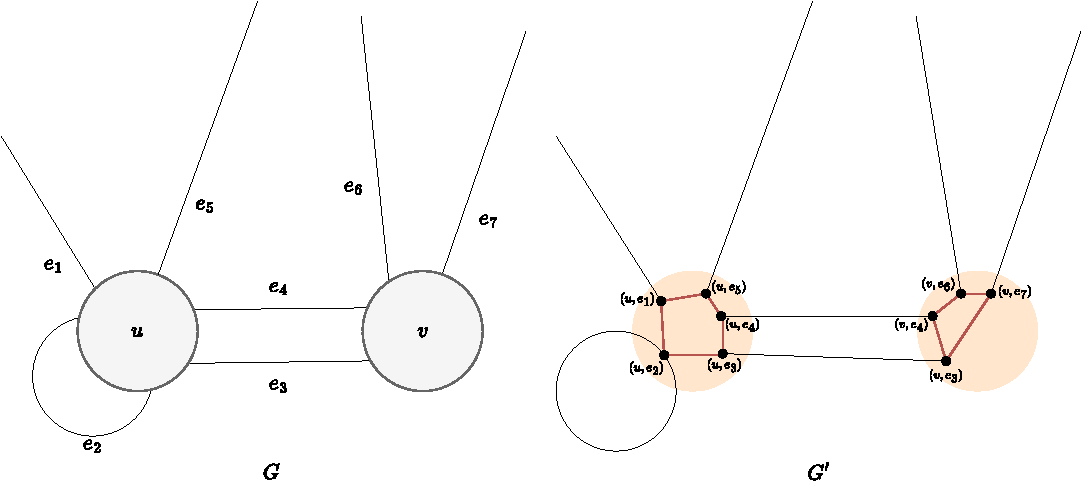
\includegraphics[width=\textwidth]{images/degree_reduction.pdf}
  \caption{次数削減変換の例. 橙色の内部の頂点集合がクラウドであり, クラウド内の辺は\cref{thm:construction-of-expander-graph}によって構成されるが, ここでは図の簡単のため$X_d$を長さ$d$の閉路としている. $G'$における黒い辺の制約は対応する元のグラフの辺と同一の制約とし, クラウド内の赤辺の制約は等式制約とする.}
  \label{fig:degree-reduction}
\end{figure}

元のグラフの各頂点$u\in V$に対し, 
\[[u]=\qty{ (u,e) \in \{u\}\times E \colon e=\{u,v\} \text{ for some } v\in V }\]
を(この証明のローカルな用語として)\emph{$u$-クラウド}と呼ぶことにする.
新しい頂点集合$V'$は$V'=\bigcup_{u\in V} [u]$である.
すなわち, $u$をそれに接続する辺の本数(自己ループは1個分としてカウント)だけコピーして得られる集合が$[u]$である.

次に辺集合$E'$を以下のように構成する.
まず, $(X_n)_{n\in\Nat}$を\cref{thm:construction-of-expander-graph}によって構成される$n$頂点$d_0$-正則$\lambda$-エクスパンダーの族とする.
元のグラフの各頂点$u\in V$に対し, $d=\abs{[u]}$としたとき, 頂点集合$[u]$上で$X_d$と同型なグラフを構成し, それを$([u],E_u)$とする.
このとき, 各$u$-クラウド内部の辺集合$E_{\mathrm{inner}}$は
\begin{align*}
  E_{\mathrm{inner}} = \bigcup_{u\in V} E_u
\end{align*}
とする.
次に異なるクラウド間を繋ぐ辺集合$E_{\mathrm{outer}}$を
\begin{align*}
  E_{\mathrm{outer}} = \qty{\qty{ (u,e), (v,e) } \colon e\notin [u]\cap[v]}
\end{align*}
とする.
このとき, グラフ$G'$の辺集合$E'$は
\begin{align*}
  E' = E_{\mathrm{inner}} \cup E_{\mathrm{outer}}
\end{align*}
となる.

次に各辺$e'\in E'$の制約$c'_{e'}$を以下のように定める:
\begin{itemize}
\item 辺$e'\in E_{\mathrm{outer}}$がクラウド間をつなぐ辺ならば, その制約は対応する元の辺$e$の制約と同じとする.
すなわち, $e'=\qty{ (u,e), (v,e) }$ならば, $c'_{e'}=c_e$である.
\item 辺$e'\in E_{\mathrm{inner}}$がクラウド内部の辺ならば, その制約を$c'_{e'}=\{(\sigma,\sigma)\colon \sigma\in\Sigma\}$, すなわち等式制約とする.
\end{itemize}

このようにして得られる制約グラフ$G'=\ip{(V',E'),\Sigma,\calC'}$が補題の主張を全て満たすことを確認する.
まず, $G'$は$(d_0+1)$-正則である.
実際, $G'$の各頂点$(u,e)\in V'$に接続する辺は, クラウド内の辺が$d_0$本, クラウド間の辺が$1$本である.
また, $G$から$G'$を構成する際に新たに追加する辺は$E_{\mathrm{inner}}$のみであり, これは高々$\sum_{u\in V}\frac{d_0\deg_G(u)}{2} \le d_0\abs{E}$本である (ここで\cref{eq:hand_shake_multigraph}を用いた).
従って
\begin{align}
  \abs{E'} = \abs{E_{\mathrm{inner}}} + \abs{E_{\mathrm{outer}}} \le \qty(d_0+1)\abs{E} \label{eq:bound_of_E'}
\end{align}
を満たす.
また, $V'$の要素数は次数の総和に等しいため, $\abs{V'}\le 2\abs{E}$を満たす.
次に, $\UNSAT(G)=0$ならば$\UNSAT(G')=0$である.
実際, 元の制約グラフの全ての制約を満たす割り当て$a\colon V\to\Sigma$に対し, $G'$の割り当て$a'\colon V'\to\Sigma$を
\begin{align*}
  a'(u,e) = a(u)
\end{align*}
と定めると, $a'$は$G'$の制約を満たす (同一クラウド内の頂点には全て同じ値が割り当てられるため, クラウド内の辺の制約は全て満たされ, クラウド間の辺に対応する制約は$a$の取り方により全て満たされることがわかる).

最後の主張, すなわち$\UNSAT(G') \ge c'\cdot \UNSAT(G)$となる定数$c'>0$が存在すること示す.
定数$c'>0$を
\begin{align}
  c' = \min\qty{\frac{(1-\lambda_0)d_0}{8(d_0+1)}, \frac{1}{2(d_0+1)}} \label{eq:c_of_degree_reduction}
\end{align}
と定める.
$\UNSAT(a';G')=\UNSAT(G')$を満たす割り当て$a'\colon V'\to\Sigma$を任意に取る.
この割り当て$a'$に対し, 元のグラフ$G$の割り当て$a\colon V\to\Sigma$を
\begin{align*}
  a(u) = \Maj((a'(u,e))_{(u,e) \in [u]})
\end{align*}
と定める. ここで$\Maj(\cdot)$は多数決関数であり,
タイは任意に選ぶとする.
例えば$\Maj(1,2,2)=2$, $\Maj(1,2,3,3)=3$, $\Maj(1,2,2,3,3)=2$である ($\Maj(1,2,2,3,3)=3$としても良いが, ここでは便宜上小さい方の数字を採用している).

以降, 割り当て$a'\colon V'\to\Sigma$に対し, 頂点$(u,e)\in V'$への割り当て$a'(u,e)$を頂点$(u,e)$の\emph{意見}と呼ぶこととする.
同様に, 割り当て$a\colon V\to\Sigma$に対し, 頂点$u\in V$への割り当て$a(u)$を頂点$u$の意見と呼ぶこととする.
直感的には頂点$u$の意見は対応する$u$-クラウド内の頂点の意見の多数決である.


辺集合$F\subseteq E$を割り当て$a$によって充足されない辺の集合, すなわち
\begin{align*}
  F = \qty{ e=\{u,v\}\in E \colon (a(u),a(v)) \not\in c_e}
\end{align*}
と定義する.
ここで$\calC = (c_e)_{e\in E}$は元の制約グラフ$G$の制約である.
同様に, $F'\subseteq E'$を割り当て$a'$によって充足されない辺の集合とする.
このとき$\UNSAT(a;G) = \frac{|F|}{|E|}$および$\UNSAT((a';G') = \frac{|F'|}{|E'|}$である.
頂点部分集合$S\subseteq V'$を$a$の多数決で選ばれなかった意見を持つ頂点の集合, すなわち
\begin{align*}
  S = \qty{ (u,e) \in V' \colon a(u) \ne a'(u,e)}
\end{align*}
と定義し, 各$v\in V$に対し$S^v = S\cap [v]$とし, 各$\sigma\in \Sigma$に対し$S^v_\sigma = \qty{ (u,e)\in S^v \colon a'(u,e)=\sigma }$とする (\cref{fig:majority-degree-reduction}).
なお, $\sigma\in\Sigma$が多数決の意見 (すなわち$\sigma=a(v)$)のとき, $S^v_\sigma=\emptyset$とする.

\begin{figure}[ht]
  \centering
  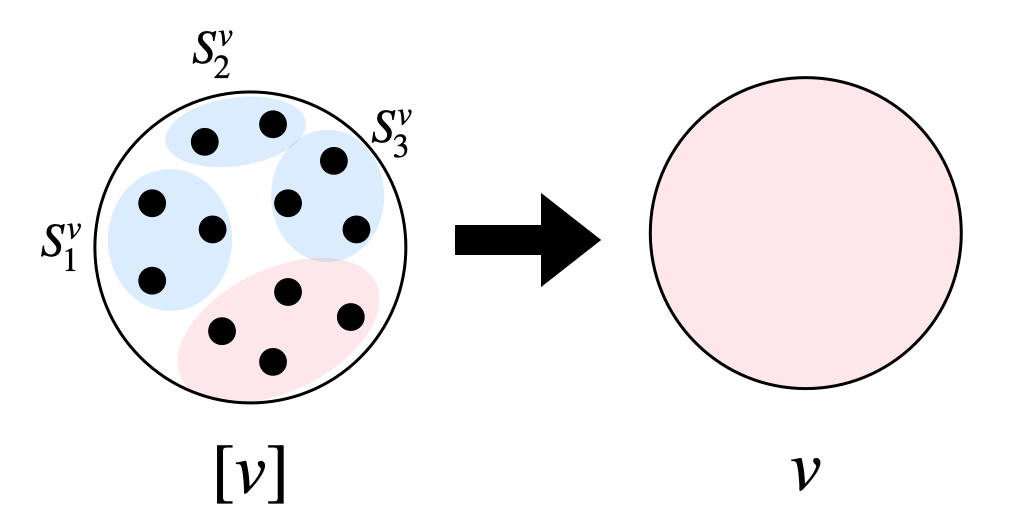
\includegraphics[width=\textwidth]{images/majority_degree_reduction.png}
  \caption{多数決によって選ばれなかった$v$-クラウド内の頂点の集合を$S_v\subseteq [v]$とする. \label{fig:majority-degree-reduction}}
\end{figure}

以下の二つのケースを考える:

\paragraph*{ケース1. $\abs{S} \ge \frac{\UNSAT(a;G)}{2}\abs{E}$の場合.}

各頂点$v\in V$と多数決によって選ばれなかった意見$\sigma\in\Sigma \setminus \{a(v)\}$に対し$\abs{S^v_\sigma} \le \frac{\abs{[v]}}{2}$である
(そうでなければ意見$\sigma$が多数決によって選ばれなかったことに矛盾する).
ここで$v$-クラウド内部のグラフは$d_0$-正則$\lambda_0$-エクスパンダーであるため, その頂点部分集合$S^v_\sigma\subseteq[v]$に対するエクスパンダー混交補題(\cref{lem:expander-mixing-lemma})より,
\begin{align*}
  W(S^v_\sigma, [v]\setminus S^v_\sigma) \ge (1-\lambda_0)\cdot \frac{d_0\abs{S^v_\sigma}}{2}
\end{align*}
となる. ここで$W(S,T)$は$v$-クラウド内部のグラフ$([v],E_v)$の辺であって$S$と$T$の間をまたがる辺の本数である.
ここで$S^v_\sigma$と$[v]\setminus S^v_\sigma$をまたがる全ての辺の両端点の意見は異なるため, $a'$はこれらの辺を充足しない. よってこれらの辺は全て$F'$に含まれる.
従って
\begin{align*}
  \abs{F'} &\ge \frac{1}{2}\sum_{v,\sigma} W(S^v_\sigma, [v]\setminus S^v_\sigma) \\
  &\ge \frac{(1-\lambda_0)d_0}{4}\sum_{v,\sigma} \abs{S^v_\sigma} \\
  &= \frac{(1-\lambda_0)d_0}{4}\abs{S} \\
  &\ge \frac{(1-\lambda_0)d_0}{8}\UNSAT(a;G)\cdot \abs{E}  & & \because \text{ケース1の仮定} \\
  &\ge \frac{(1-\lambda_0)d_0}{8(d_0+1)}\UNSAT(a;G)\cdot \abs{E'}. & & \because\text{\cref{eq:bound_of_E'}}
\end{align*}
特にこれから$\UNSAT(a';G') = \frac{\abs{F'}}{\abs{E'}}\ge \frac{(1-\lambda_0)d_0}{8(d_0+1)}\cdot\UNSAT(a;G)$が成り立つ.

\paragraph*{ケース2. $\abs{S} < \frac{\UNSAT(a;G)}{2}\abs{E}$の場合.}
任意の辺$e = \{u,v\} \in F$に対して, それに対応する$G'$の辺$e' = \{(u,e),(v,e)\}$を考える.
\begin{itemize}
\item もしも$a(u)=a'(u,e)$かつ$a(v)=a'(v,e)$が成り立つならば, $e'$と$e$は同じ制約を持ち, $e\in F$であることから$e'\in F'$である.
\item そうでない, すなわち$a(u)\ne a'(u,e)$または$a(v)\ne a'(v,e)$が成り立つならば, $(u,e)$と$(v,e)$のうち少なくとも一方はその意見が多数決として選ばれない, すなわち$(u,e)\in S$または$(v,e)\in S$が成り立つ.
\end{itemize}
以上より$\abs{F} \le \abs{F'} + \abs{S}$が成り立つので
\begin{align*}
  \abs{F'} &\ge \abs{F} - \abs{S} \\
  &\ge \abs{E}\UNSAT(a;G) - \frac{\UNSAT(a;G)}{2}\abs{E} & & \because \text{ケース2の仮定}\\
  &= \frac{\UNSAT(a;G)}{2}\abs{E} \\
  &\ge \frac{\UNSAT(a;G)}{2(d_0+1)}\abs{E'} & & \because\text{\cref{eq:bound_of_E'}}
\end{align*}
となり, これから
\begin{align*}
  \UNSAT(a';G') = \frac{\abs{F'}}{\abs{E'}} \ge \frac{1}{2(d_0+1)}\cdot \UNSAT(a;G)
\end{align*}
が成り立つ.

ケース1,2より, \cref{eq:c_of_degree_reduction}で定まる定数$c'>0$に対して$\UNSAT(a';G') \ge c'\cdot \UNSAT(a;G) \ge c'\cdot \UNSAT(G)$が成り立つ.
\end{proof}

\subsection{エクスパンダー化}

次に, 与えられた正則な制約グラフをエクスパンダーグラフに変換する補題を示す.

\begin{lemma}{エクスパンダー化補題}{expanderization}
ある定数$\lambda<1,d,d_0\in\Nat$および次を満たす多項式時間アルゴリズム$A$が存在する:
アルゴリズム$A$は入力として$d$-正則な制約グラフ$G = \ip{ (V,E), \Sigma, \calC }$
を受け取り, $(d+d_0+1)$-正則で全頂点が自己ループを持ち, さらに$\lambda$-エクスパンダーである制約グラフ $G' = \ip{ (V, E'), \Sigma, \calC' }$ を出力する.
さらに, この制約グラフ$G'$は$\UNSAT(G') = \frac{d}{d+d_0+1}\UNSAT(G)$を満たす.
\end{lemma}

\begin{proof}
入力として与えられた制約グラフを$G=\ip{(V,E),\Sigma,\calC}$とする.
変換は以下のようにして行われる:
\begin{enumerate}
\item まず, \cref{thm:construction-of-expander-graph}を用いて頂点集合$V$上$d_0$-正則$\lambda_0$-エクスパンダーグラフを構成し, その辺集合を$E$に追加する (この際多重辺も許す).
\item 次に, 各頂点に自己ループを付与する.
\item ステップ1,2で追加した辺$e$に対応する制約$c'_e$を自明な制約$c'_e=\Sigma^2$とする.
\end{enumerate}
このようにして得られる制約グラフを$G'=\ip{(V',E'),\Sigma,\calC'}$とする.
元の制約グラフ$G$が$d$-正則であることから, $G'$は$(d+d_0+1)$-正則である (自己ループの次数への寄与は$1$であることに注意).
また, ステップ2より$G'$は全頂点が自己ループを持つ.

次に$\UNSAT(G')=\frac{d}{d+d_0+1}\UNSAT(G)$を示す.
任意の割り当て$a\colon V \to \Sigma$に対し, 
ステップ1,2で追加した辺に対応する制約は常に充足されるため, 両者が充足\emph{しない}制約の個数は一致する.
すなわち$\abs{E}\UNSAT(a;G) = \abs{E'}\UNSAT(a;G')$が成り立つので
\begin{align*}
  \UNSAT(G') = \min_{a}\UNSAT(a;G') = \frac{\abs{E}}{\abs{E'}}\min_a \UNSAT(a;G) = \frac{d}{d+d_0+1}\UNSAT(G)
\end{align*}
が成り立つ.

最後に$G'$が$\lambda:=\frac{d}{d+d_0+1}+\frac{\lambda_0(d_0+1)}{d+d_0+1}$に対し$\lambda$-エクスパンダーであることを示す.
元のグラフ$G$の遷移確率行列を$P\in[0,1]^{V\times V}$とし,
ステップ1,2で追加した辺からなるグラフを$G_0$とし, その遷移確率行列を$P_0\in[0,1]^{V\times V}$とする.
また, 最終的に得られるグラフ$G'$の遷移確率行列を$P'\in[0,1]^{V\times V}$とする.
元のグラフ$G$は$d$-正則, 追加したグラフ$G_0$は$(d_0+1)$-正則であるため
\begin{align*}
  P' = \frac{d}{d+d_0+1}P + \frac{d_0+1}{d+d_0+1}P_0
\end{align*}
となる.
さらに$P_0$は$\lambda_0$-エクスパンダーであるため, 全成分$1$のベクトル$\allone$と直交する任意のベクトル$x\in \Real^V$に対し
\begin{align*}
  x^\top P' x &= \frac{d}{d+d_0+1}x^\top P x + \frac{d_0+1}{d+d_0+1}x^\top P_0 x \\
  &\ge \frac{d}{d+d_0+1}\norm{x}^2 + \frac{d_0+1}{d+d_0+1}\lambda_0\norm{x}^2 & & \because\text{$P_0$のエクスパンダー性}\\
  &\le \qty( \frac{d}{d+d_0+1} + \frac{\lambda_0(d_0+1)}{d+d_0+1} )\norm{x}^2
\end{align*}
より, $\lambda(P')\le \frac{d}{d+d_0+1} + \frac{\lambda_0(d_0+1)}{d+d_0+1}$が成り立つ.
\end{proof}

これにより\cref{lem:constant-degree-expanderization}を示す準備が整った.
\begin{proof}[\cref{lem:constant-degree-expanderization}の証明]

与えられた制約グラフ$G$に対し, まず$G$を入力として\cref{lem:degree-reduction}のアルゴリズムを実行し, その出力を$G_1$とする.
この制約グラフ$G_1$は\cref{lem:degree-reduction}の主張より, $d$-正則である.
次に, $G_1$を入力として\cref{lem:expanderization}のアルゴリズムを実行し, その出力を最終的な出力$G$とする.
この制約グラフ$G'$は\cref{lem:expanderization}の主張より, 全頂点が自己ループを持ち, $(d+d_0+1)$-正則かつ$\lambda$-エクスパンダーである.
また, この一連の変換によって$\size(G')$は$\size(G)$の定数倍にしかならない.

最後に$\UNSAT$の値を考える.
元の制約グラフ$G$が$\UNSAT(G)=0$ならば, \cref{lem:degree-reduction,lem:expanderization}より
$\UNSAT(G') = \frac{d}{d+d_0+1}\UNSAT(G_1) = 0$を得る.
一方で
\begin{align*}
  \UNSAT(G') = \frac{d}{d+d_0+1}\UNSAT(G_1) \ge \frac{d}{d+d_0+1}\cdot c'\cdot\UNSAT(G).
\end{align*}
すなわち$\beta = \frac{d}{d+d_0+1}\cdot c'$に対して主張が成り立つことが示された.
\end{proof}

\section{制約グラフのべき乗}

\cref{lem:constant-degree-expanderization}により, 任意の制約グラフを定数次数エクスパンダーに変換することができる.
この節では, そのような制約グラフに対し, 以下で定義する\emph{べき乗}という操作を考えることで, その$\UNSAT$の値を増幅させることができることを示す.

\begin{definition}{制約グラフの冪乗}{power-of-constraint-graph}
  パラメータ$\ell\in\Nat$および全頂点が自己ループを持つ$d$-正則な制約グラフ$G=\ip{(V,E),\Sigma,\calC}$に対し, べき乗$G^\ell = \ip{(V,\boldE),\Sigma^{d^{\ell}},\calC^\ell}$を, 以下のようにして定義する:
  \begin{itemize}
    \item 頂点集合は同じ$V$とする. なお, $V$の元は$v_1<\dots < v_n$のように順序づけられているとする.
    \item グラフ$(V,\boldE)$をべき乗(\cref{def:power-of-graph})によって得られるグラフ$(V,E)^\ell$とする. すなわち, 各二頂点$u,v\in V$に対し, 長さ$\ell$の$uv$-路の個数と同じだけ$uv$間に多重辺を用意する ($uv$-路と$vu$路の個数は一致するため, 無向グラフとして定義できる). このようにして得られる辺の多重集合を$\boldE$とし, その元を$\bolde = \{u,v\} \in \boldE$とする.
    \item アルファベット集合は$\Sigma^{d^{\ell}}$とする. ここで, 頂点$u$に$\vec{\sigma}=(\sigma_1,\dots,\sigma_{d^{\ell}}) \in \Sigma^{d^{\ell}}$が割り当てられたとき, 次の意味を持つ: 元の$d$-正則グラフ$G$上で頂点$u$から距離$\ell$以内の頂点の集合を$\Gamma(u)$とし\footnote{頂点$v$が頂点$u$から距離$i$以内であるというのは, 頂点$u$から開始し頂点$v$に至る長さ$i$以下の路が存在することをいう.}, その元を頂点番号の大小順で並べて$\Gamma(u)=\qty{ v_1,\dots,v_\ell}$ とする (ここで$G$の$d$-正則性より$\ell \le d^{\ell}$である). このとき, $\vec{\sigma}$は各$v\in\Gamma(u)$に$\vec{\sigma}_u\in \Sigma$を割り当てる写像とみなし, $\vec{\sigma}_v$を\emph{$u$の$v$に対する意見}と呼ぶ.
    なお, $\ell < d^{\ell}$の場合は相異なる二つの$\vec{\sigma},\vec{\sigma}'\in\Sigma^{d^{\ell}}$が同一の写像としてみなされることもある (これらは制約を充足するか否かにおいては区別されない).
    \item 辺$\bolde = \{u,v\} \in \boldE$ に対応する制約$\boldc_{\bolde}\in \calC^\ell$は次の二つを満たす割り当て$(\vec{\sigma},\vec{\sigma}')\in \Sigma^{d^{\ell}} \times \Sigma^{d^{\ell}}$によって満たされる:
    元のグラフ$G$の全ての辺$e=\{s,t\}\in E$ (ただし$s<t$)に対し,
      \begin{itemize}
        \item $s\in \Gamma(u), t\in\Gamma(v)$ならば$(\vec{\sigma}(s), \vec{\sigma}'(t))\in c_e$が成り立つ.
        \item $s\in\Gamma(v), t\in\Gamma(u)$ならば$(\vec{\sigma}'(s), \vec{\sigma}(t))\in c_e$が成り立つ.
      \end{itemize}
  \end{itemize}
\end{definition}

\begin{figure}[ht]
  \centering
  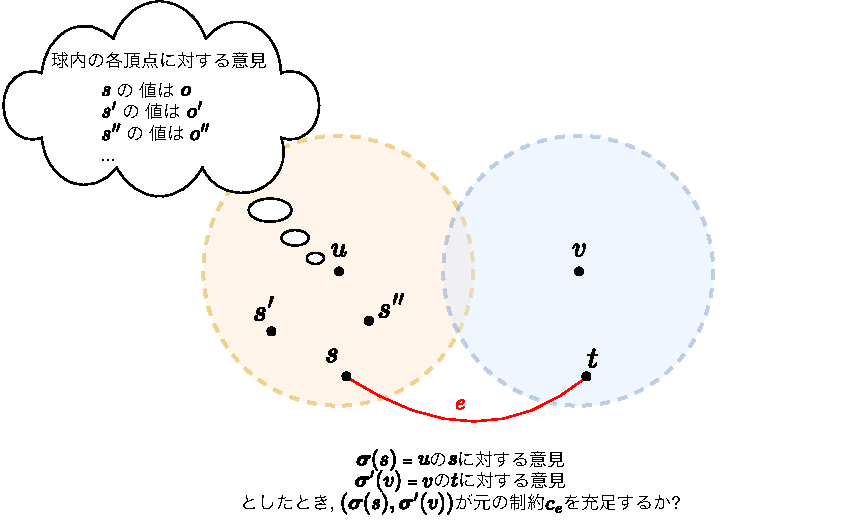
\includegraphics[width=\textwidth]{images/gap_amplification.pdf}
  \caption{制約グラフ$G$のべき乗$G^\ell$の図例. 頂点$u,v$にそれぞれ$\vec{\sigma},\vec{\sigma}'\in\Sigma^{d^{\ell}}$が割り当てられているとき, それぞれ関数$\vec{\sigma}\colon \Gamma(u)\to\Sigma$と$\vec{\sigma}'\colon \Gamma(v)\to\Sigma$とみなす. なお, 元のグラフ$G$が自己ループを持つことから, 距離$\ell$以内の全ての頂点に対して意見が定義される.\label{fig:gap-amplification}}
\end{figure}

最後に, $G^\ell$における割り当て$a'\colon V\to\Sigma^{d^{\ell}}$に対し, $u$の$w$に対する意見を$a'(u)_w$と表すことにする.

パラメータ$\ell$は制約グラフのサイズ$\size(G)$には依存しない定数であることを常に想定する.
べき乗をで得られた制約グラフは元の制約グラフに対して$\UNSAT$の値が増幅している.

\begin{lemma}{べき乗の性質}{property-of-power}
  ある定数$\beta=\beta(\lambda,d,\abs{\Sigma})$が存在して以下が成り立つ:
  十分大きいパラメータ$\ell=\ell(d,\abs{\Sigma},\lambda) \le \abs{E}$および全頂点が自己ループを持つ$d$-正則な制約グラフ$G=\ip{(V,E),\Sigma,\calC}$に対し, べき乗$G^\ell = \ip{(V,\boldE),\Sigma^{\ell},\calC^\ell}$を, \cref{def:power-of-constraint-graph}で定義する.
  このとき
  \begin{itemize}
    \item $\size(G^\ell) \le \size(G)\cdot d^\ell$である.
    \item $\UNSAT(G)=0$ならば$\UNSAT(G^\ell)=0$である.
    \item $\UNSAT(G^\ell) \ge \beta\sqrt{\ell}\cdot \min\qty{ \UNSAT(G), \frac{1}{\ell} }$である.
  \end{itemize}
\end{lemma}

\begin{remark}{「定数」の意味}{mean-of-constants}
  主張や証明の中でしばし「定数」という言葉を多用するが, ここでは$d,\lambda,\abs{\Sigma}$をユニバーサルな定数で固定し, これらの値に応じて定まる値$\beta,\ell$なども定数と呼ぶ.
  ただし, 定数はグラフの頂点数や辺数には依存しない.
\end{remark}

\begin{proof}

定義より$\abs{\boldE} \le \abs{V}d^{\ell}$であるから, $\size(G^\ell) \le \size(G)\cdot d^\ell$である.

また, $\UNSAT(G)=0$ならば, 全制約を満たす割り当て$a\colon V \to \Sigma$に対し, $a'(u)$に
\begin{align*}
  \vec{\sigma}(u)\colon w \mapsto a(w)
\end{align*}
で定まる関数$\vec{\sigma}\colon \Gamma(w)\to\Sigma$とみなせる値$\vec{\sigma}\in\Sigma^{d^\ell}$を割り当てる (候補が複数存在する場合はどれでもよい).
このようにして定まる$a'\colon V\to\Sigma^{\ell}$を考えると, これは全ての制約を満たす割り当てであるため, $\UNSAT(G^\ell)=0$である.

最後に$\UNSAT(G^\ell)$の下界を証明する.
簡単のため$\ell$は偶数であるとする (奇数の場合は$\ell/2$を$\floor{\ell/2}$に置き換えれば同じ証明が成立する).
頂点$u\in V$に対し, $V$値をとる確率変数$\RW_j(u)$を, グラフ$G$上で頂点$u$から開始する長さ$j$のランダムウォークの最終到達頂点とする (長さとは辿った辺の本数のことである).
べき乗の制約グラフ$G^\ell$における割り当て$a'\colon V \to \Sigma^{\ell}$に対し, 元の制約グラフに対する任意の割り当て$a\colon V\to\Sigma$を
\begin{align}
  a(u) = \argmax_{\tau \in \Sigma} \qty{ \Pr\qty[ a'(\RW_{\ell/2}(u))_u = \tau ] }. \label{eq:argmax-of-RW}
\end{align}
によって定める.
常に$\RW_{\ell/2}(u)\in \Gamma(u)$であるから$a'(\RW(u))_u$は必ず存在する.
すなわち, $u$から開始したランダムウォークが最も「拾いやすい」意見を$a(u)$としている.
このようにして定めた割り当て$a\colon V \to \Sigma$は, 適当な定数$\beta=\beta(\lambda,d,\abs{\Sigma})>0$に対して
\begin{align}
  \UNSAT(a';G^\ell) \ge \beta\sqrt{\ell}\cdot \min\qty{ \UNSAT(a;G), \frac{1}{\ell} }. \label{eq:lower-bound-of-UNSAT}
\end{align}
を満たすことを後で示す. $\UNSAT(a';G^\ell)=\UNSAT(G^\ell)$を満たす$a'$に対して\cref{eq:lower-bound-of-UNSAT}を適用し, さらに$\UNSAT(a;G)\le \UNSAT(G)$を代入すると$\UNSAT(G^\ell)$の所望の下界が得られて証明は完了する.

\paragraph*{\cref{eq:lower-bound-of-UNSAT}の証明.}

割り当て$a'\colon V\to \Sigma^{d^{\ell}}$を固定し, $a$を\cref{eq:argmax-of-RW}によって定める.
辺部分集合$F_0\subseteq E$を, $a$によって充足されない辺の集合とし,
さらにその部分集合$F\subseteq F_0$を, 
\begin{itemize}
\item $\abs{F_0} \le \frac{\abs{E}}{\ell}$ならば$F_0=F$,
\item そうでない場合は$\abs{F} = \floor*{\frac{\abs{E}}{\ell}}$となるように$F$を任意に固定する.
\end{itemize}
このとき, 任意の$x\ge 1$に対し$\floor{x}\ge x/2$であることから, $\frac{\abs{E}}{\ell}\ge 1$の仮定を用いて
\begin{align}
  \abs{F} &\ge \min\qty{ \abs{F_0}, \floor*{\frac{\abs{E}}{\ell}} } \nonumber \\
  &\ge \frac{1}{2}\min\qty{ \abs{F_0}, \frac{\abs{E}}{\ell} } \nonumber \\
  &\ge \frac{\abs{E}}{2}\min\qty{ \UNSAT(a;G), \frac{1}{\ell} } \label{eq:abs-F}
\end{align}
を得る (なお, $\abs{E}\ge \ell$の仮定を用いるのはここのみである).

べき乗グラフの辺$\bolde \in \boldE$は$G$上の長さ$\ell$の路に対応する.
従って$\bolde = (u_0,\dots,u_\ell)$ (ただし全ての$i\in[\ell]$に対し$\qty{u_{i-1},u_{i}}\in E$)と表し, 元のグラフの辺と区別するため$e\in E$を$G$辺, $\bolde\in\boldE$を$G^\ell$辺と呼ぶことにする.

$G^\ell$辺$\bolde=(u_0,\dots,u_\ell)$の$i$番目の辺$e_i:=\qty{u_{i-1},u_i}$は
\begin{itemize}
  \item $e_i \in F$
  \item $a'(u_{0})_{u_{i-1}} = a(u_{i-1})$ かつ $a'(u_\ell)_{u_i} = a(u_i)$
\end{itemize}
をどちらも満たすとき, \emph{悪い}ということにする.
一様ランダムに$\bolde$を選んだとき, $B_i\in\binset$を辺$e_i$が悪いならば$B_i=1$, そうでないならば$B_i=0$とする (これらは確率変数である).
さらに
\begin{align*}
  I = \qty[\frac{\ell}{2} - \sqrt{\ell}, \frac{\ell}{2} + \sqrt{\ell}] \cap \mathbb{Z}
\end{align*}
に対し, $B=\sum_{i\in I}B_i$とする.
もしも$B>0$ならば, 辺$\bolde$の制約$c'_{\bolde}$は$a'$によって充足されない.
従って, $\UNSAT(a';G^\ell) \ge \Pr_{\bolde\sim \boldE}[B\ge 1]$である.

Paley-Zygmundの不等式(\cref{lem:paley-zigmund-inequality})より, $\E[B]$および$\E[B^2]$を評価することで$\Pr[B\ge 1]$の下界を得ることができる.
これらは以下のように評価できる. 

\begin{claim}{$B$の期待値}{expectation-of-B}
  ある十分小さな定数$C=C(d,\lambda,\abs{\Sigma})>0$が存在して, $B$の期待値は
  \begin{align*}
    \E[B] \ge C\sqrt{\ell} \cdot \frac{\abs{F}}{\abs{E}}.
  \end{align*}
\end{claim}

\begin{claim}{$B^2$の期待値}{expectation-of-B-squared}
  ある十分大きな定数$C'=C'(d,\lambda,\abs{\Sigma})>0$が存在して, $B^2$の期待値は
  \begin{align*}
    \E[B^2] \le C'\sqrt{\ell} \cdot \frac{\abs{F}}{\abs{E}}.
  \end{align*}
\end{claim}

これらの主張の証明は後で与える.
ここでは, これらを用いて\cref{eq:lower-bound-of-UNSAT}を示す.
実際, \cref{lem:paley-zigmund-inequality,claim:expectation-of-B,claim:expectation-of-B-squared}より, 定数$\beta=\frac{C^2}{2C'}>0$に対して
\begin{align*}
  \UNSAT(a';G^\ell) &\ge \Pr[B\ge 1] \\
  &\ge \frac{\E[B]^2}{\E[B^2]} \\
  &\ge \frac{C^2}{C'} \sqrt{\ell} \cdot \frac{\abs{F}}{\abs{E}} \\
  & \ge \beta \sqrt{\ell} \cdot \min\qty{ \UNSAT(a;G), \frac{1}{\ell} } & & \because \text{\cref{eq:abs-F}}
\end{align*}
となり主張を得る.

\end{proof}

最後に残された二つの主張の証明を与える. なお, 制約グラフのエクスパンダー性を用いるのは\cref{claim:expectation-of-B-squared}の証明のみである.
\begin{proof}[\cref{claim:expectation-of-B}の証明]
  各$i\in I$に対して$\E[B_i]=\Pr_{\bolde\sim \boldE}[e_i\text{ が悪い}]$を下から抑えればよい.
  一様ランダムな$\bolde=(u_0,\dots,u_\ell)\sim\boldE$は$G$上の長さ$\ell$のランダムウォークであるから, 各$i\in I$に対して$\bolde$は以下のプロセスによって生成される:
  \begin{enumerate}
    \item 辺$\{u_{i-1},u_i\}\sim E$を一様ランダムに選ぶ.
    \item 頂点$u_{i-1}$から開始して長さ$i-1$のランダムウォークを行い, 辿った頂点を順番に$u_{i-1},u_{i-2},\dots,u_0$とする.
    \item 同様に, 頂点$u_i$から開始して長さ$\ell-i$のランダムウォークを行い, 辿った頂点を順番に$u_i,u_{i+1},\dots,u_\ell$とする.
    \item 頂点列$(u_0,\dots,u_\ell)$に対応する$\bolde \in \boldE$を出力する.
  \end{enumerate}

  \begin{figure}[ht]
    \centering
    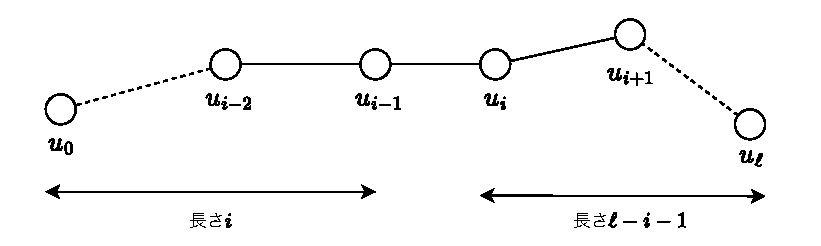
\includegraphics[width=0.9\textwidth]{images/randomwalk_process.pdf}
    \caption{ランダムウォークの図例. 頂点$u_0$から開始して長さ$i-1$のランダムウォークを行い, 辿った頂点を順番に$u_{i-1},u_{i-2},\dots,u_0$とする. 同様に, 頂点$u_i$から開始して長さ$\ell-i$のランダムウォークを行い, 辿った頂点を順番に$u_i,u_{i+1},\dots,u_\ell$とする. この二つのランダムウォークを組み合わせて, 長さ$\ell$のランダムウォークを生成する. \label{fig:random-walk}}
  \end{figure}

  このプロセスに基づいて, $\Pr[B_i=1]$を評価する.
  まず, ステップ1で選ばれた辺が$\qty{u_{i-1},u_i}\in F$である確率は$\frac{\abs{F}}{\abs{E}}$である.
  次にステップ1で選ばれた辺$\qty{u_{i-1},u_i}\in F$で条件つけたとき, ステップ2と3は独立なランダムネスに基づく試行であるため, それぞれの両端点$u_0,u_\ell$は独立な確率変数である.
  従って
  \begin{align}
    \Pr[B_i=1] &= \E_{\text{step 1-3}}\qty[\{u_{i-1},u_i\}\in F \text{ and }a'(u_0)_{u_{i-1}} = a(u_{i-1})\text{ and }a'(u_\ell)_{u_i} = a(u_i)] \nonumber \\
     &= \frac{\abs{F}}{\abs{E}} \cdot \E_{\{u_{i-1},u_i\}\sim F}\qty[ \underbrace{\Pr_{\text{step 2}}[a'(u_0)_{u_{i-1}} = a(u_{i-1})]}_{=:p_0} \cdot \underbrace{\Pr_{\text{step 3}}[a'(u_\ell)_{u_i} = a(u_i)]}_{=:p_\ell}] \label{eq:Pr-B_i}
  \end{align}
  を得る. 二つ目の等式では, $\{u_{i-1},u_i\}\in F$で条件つけて$\{u_{i-1},u_i\}\sim E$をランダムに選ぶというのは, $F$内の辺を一様ランダムに選ぶことに他ならないことに留意する.

  次に, $p_0$と$p_\ell$を評価する.
  頂点$u_{i-1}$を任意に固定して$p_0$を考える ($p_\ell$も同様に示せる).
  頂点$u\in V$および非負整数$m\ge 0$に対し, 確率変数$X_{u,m}\in\Sigma$を, ($a'$における)$\RW_m(u)$の$u$に対する意見, すなわち$X_{u,m} = a'(\RW_m(u))_u$とする.
  \cref{eq:argmax-of-RW}より, $m=\ell/2$のとき, 
  \begin{align}
  \Pr[X_{u_{i-1},\ell/2} = a(u_{i-1})] \ge \frac{1}{\abs{\Sigma}} \label{eq:center_opinion}
  \end{align}
  である.
  ステップ2で選ばれた端点$u_0$は$u_0=\RW_i(u_{i-1})$であるから, $X_{u_{i-1},i}=a'\qty( \RW_i(u_{i-1}) )_{u_{i-1}} = a'\qty(u_0)_{u_{i-1}}$である.
  従って, 
  \begin{align}
    p_0 = \Pr[X_{u_{i-1},i} = a(u_{i-1})] \label{eq:p_0}
  \end{align}
  である. 任意に頂点$u\in V$と$i\in I$を固定して$X_{u,\ell/2}$と$X_{u,i}$の分布を比較する.
  $i\in I$なので, $\abs{i-\ell/2} \le \sqrt{\ell}$である.

  元のグラフ$G$の各頂点に対し, その頂点が持つ自己ループの一つを赤く塗る
  (仮定より元のグラフ$(V,E)$は$d$-正則かつ各頂点が自己ループを少なくとも一つ持つ).
  頂点$u$から開始する長さ$\ell/2$のランダムウォークを考え,
  確率変数$Y_{\ell/2}$を, このランダムウォークが辿った赤\emph{以外}の辺の個数とする ($Y_i$も同様に定義する).
  各頂点がちょうど一つの赤い自己ループを持つため,
  確率変数$Y_{\ell/2}$の分布は始点$u$に依存せず二項分布$\Bin(\ell/2,1-1/d)$である (同様に$Y_i$の分布は$\Bin(i,1-1/d)$である).
  また, $\RW'_k(u)$を, 頂点$u$から開始する赤い辺を選ばない長さ$k$のランダムウォークの最終到達頂点とする (すなわち, $G$の各頂点から赤い辺を除いて得られるグラフ上の長さ$k$のランダムウォークである).
  従って, 任意の頂点部分集合$A\subseteq V$に対し
  \begin{align}
    \Pr\qty[\RW_{i}(u)\in A] &= \sum_{k=0}^{i} \Pr\qty[\RW_{i}(u) \in A \condition Y_{i}=k] \cdot \Pr\qty[Y_{i}=k] \nonumber \\
    &= \sum_{k=0}^{i} \Pr\qty[\RW'_k(u) \in A] \cdot \Pr\qty[Y_{i}=k] \label{eq:RW_i_distribution}
  \end{align}
  が成り立つ.
  ここで, 以下の主張を後で示す:
  \begin{claim}{}{two-constants}
  十分大きな定数$C_1=C_1(d,\abs{\Sigma})>0$と十分小さな定数$C_2=C_2(d,\abs{\Sigma})>0$が存在して以下が成り立つ:
  $K:= \qty{ k\in \mathbb{Z}_{\ge 0} \colon \abs{k - \qty(1-\frac{1}{d})\frac{\ell}{2}} \le C_1\sqrt{\ell} }$ としたとき,
  \begin{enumerate}
    \item $\Pr\qty[Y_{\ell/2} \not\in K] \le \frac{1}{2\abs{\Sigma}}$.
    \item 全ての$k\in K$と全ての$i\in I$に対し, $\Pr\qty[Y_i=k] \ge C_2\cdot \Pr\qty[Y_{\ell/2}=k]$.
  \end{enumerate}
  \end{claim}
  
  \cref{claim:two-constants}を仮定し, その定数$C_1,C_2$を用いて\cref{claim:expectation-of-B}を示す.
  パラメータ$\ell$は$d$に依存して十分大きくとる.
  このとき, 任意の$i\in I$に対して$K\subseteq [0,\ell/2-\sqrt{\ell}] \subseteq [0,i]$が成り立つから
  \begin{align}
    \Pr\qty[\RW_{i}(u)\in A] &= \sum_{k=0}^{i} \Pr\qty[\RW'_{k}(u) \in A] \cdot \Pr\qty[Y_{i}=k] \nonumber\\
    &\ge \sum_{k\in K} \Pr\qty[\RW'_{k}(u) \in A] \cdot \underbrace{\Pr\qty[Y_{i}=k]}_{\ge C_2\cdot \Pr\qty[Y_{\ell/2}=k]} \nonumber\\
    &\ge C_2 \sum_{k \in K} \Pr\qty[\RW'_{k}(u) \in A] \cdot \Pr\qty[Y_{\ell/2}=k] \nonumber\\
    &\ge C_2 \qty(\sum_{0\le k \le \ell/2} \Pr\qty[\RW'_{k}(u) \in A] \cdot \Pr\qty[Y_{\ell/2}=k] - \Pr[Y_{\ell/2}\not\in K]) \nonumber\\
    &\ge C_2 \qty( \Pr\qty[ \RW_{\ell/2}(u)\in A ] - \frac{1}{2\abs{\Sigma}} ) \label{eq:RW_i_distribution_2}
  \end{align}
  を得る. ここで頂点部分集合$A\subseteq V$を
  $A = \qty{ v \in V \colon a'(v)_u = a(u) }$
  として\cref{eq:RW_i_distribution_2}を適用すると
  \begin{align*}
    \Pr\qty[X_{u,i}=a(u)] = \Pr\qty[ a'\qty(\RW_{i}(u))_u = a(u) ] = \Pr\qty[\RW_{i}(u)\in A] \ge \frac{C_2}{2\abs{\Sigma}}
  \end{align*}
  となるため, $u=u_{i-1}$とすると, \cref{eq:p_0}より
  \begin{align*}
    p_0 = \Pr\qty[X_{u_{i-1},i} = a(u_{i-1})]\ge \frac{C_2}{2\abs{\Sigma}}
  \end{align*}
  を得る.
  同様に, $p_\ell$についても, 適当な定数$C'_2>0$に対して$p_{\ell}\ge \frac{C'_2}{2\abs{\Sigma}}$が成り立つため, \cref{eq:Pr-B_i}より, 適当な定数$C_3=C_3(d,\abs{\Sigma})>0$に対して
  \begin{align*}
    \Pr[B_i=1] &\ge \frac{\abs{F}}{\abs{E}} \cdot \E_{\{u_{i-1},u_i\}\sim F}\qty[ p_0 \cdot p_\ell ] \ge C_3\cdot \frac{\abs{F}}{\abs{E}}
  \end{align*}
  を得る. 最後に$B=\sum_{i\in I}B_i$より, $\E[B]\ge C_3\sqrt{\ell}\cdot \frac{\abs{F}}{\abs{E}}$を得る.
\end{proof}

\begin{proof}[\cref{claim:two-constants}の証明]
  一つ目の主張は, $Y_{\ell/2}$の分布が二項分布$\Bin(\ell/2,1-1/d)$であることとChebyshevの不等式(\cref{lem:chebyshev-inequality})を用いれば示せる (\cref{exer:two-constants}).

  二つ目の主張を示す. すなわち, 二つの二項分布$\Bin(i,1-1/d)$と$\Bin(\ell/2,1-1/d)$を比較する.
  一つ目の主張を満たすように任意に定数$C_1>0$を固定する.
  このとき, 二つ目の主張が成り立つようにうまく$C_2>0$を選べることを示せばよい.

  一般に, 任意の$m\in\Nat$, 定数$p\in(0,1)$, $C>0$および$k\in\Nat$ (ただし$\abs{k-mp}\le C\sqrt{m}$を満たす)に対し, 
  \begin{align}
    \Pr\qty[\Bin(m,p) = k] = \frac{1}{\sqrt{2\pi m p(1-p)}} \exp\qty( - \frac{(k-mp)^2}{2m p(1-p)} ) \cdot \qty(1\pm O_{C,p}\qty(\frac{1}{m})) \label{eq:de-moivre-laplace}
  \end{align}
  が成り立つ (De Moivre-Laplaceの定理).
  特に, $\abs{k-mp}\le C\sqrt{m}$を満たすため, 右辺は$\Theta(1/\sqrt{m})$で評価できる.
  
  従って, 適当な定数$D_1,D_2>0$が存在して, $\ell$が十分大きいとき,
  \begin{align*}
    &\Pr[Y_i=k]=\Pr[\Bin(i,1-1/d)=k] \ge \frac{D_1}{\sqrt{i}}, \\
    &\Pr[Y_{\ell/2}=k]=\Pr[\Bin(\ell/2,1-1/d)=k] \le \frac{D_2}{\sqrt{\ell/2}}
  \end{align*}
  を満たす. $i\in I$より, 主張を得る.    
\end{proof}

\begin{exercise}{主張の証明}{two-constants}
  \cref{claim:two-constants}の一つ目の主張, すなわちある十分大きな定数$C_1=C_1(d,\abs{\Sigma})>0$が存在して
  \begin{align*}
    \Pr\qty[Y_{\ell/2} \not\in K] \le \frac{1}{2\abs{\Sigma}}
  \end{align*}
  が成り立つことを示せ.
\end{exercise}

\begin{proof}[\cref{claim:expectation-of-B-squared}の証明]
  ランダムウォーク$\bolde=(u_0,\dots,u_\ell)\sim\boldE$に対し, 確率変数$Z_i$を, $\qty{u_{i-1},u_i}\in F$ならば$Z_i=1$, そうでなければ$Z_i=0$とする.
  このとき, $B_i\le Z_i$であるから, $Z:=\sum_{i\in I} Z_i$に対し$B\le Z$であり, 特に$\E[B^2]\le \E[Z^2]$である.
  以下, $\E[Z^2]$を評価する. まず, $\E[Z_i]=\Pr[\qty{u_{i-1},u_i}\in F]=\frac{\abs{F}}{\abs{E}}$である (ランダムウォークの$i$番目の辺の周辺分布は$E$上の一様分布だから).
  定義より
  \begin{align}
    \E[Z^2] &= \sum_{i,j\in I} \E[Z_i Z_j] = \E[Z] + 2 \sum_{i,j\in I,i<j} \E[Z_i Z_j] \nonumber \\
    &= \frac{\abs{F}}{\abs{E}} \abs{I} + 2 \sum_{i,j\in I,i<j} \E[Z_iZ_j]. \label{eq:E-Z^2}
  \end{align}
  ここで, 固定した$i<j$に対して$\E[Z_iZ_j]$を上から評価する.
  すなわち, $\lambda$-エクスパンダーグラフ上の長さ$\ell$のランダムウォーク$(u_0,\dots,u_\ell)$を考えたとき, $i$番目の辺$\qty{u_{i-1},u_i}$と$j$番目の辺$\qty{u_{j-1},u_j}$が同時に$F$に含まれる確率を評価する.
  辺部分集合$F\subseteq E$の辺に接続している頂点部分集合を$V_F:=\bigcup_{e\in F} e$とすると
  \begin{align}
    \Pr_{(u_{i-1},\dots,u_j)}\qty[\qty{u_{i-1},u_i}\in F \text{ and } \qty{u_{j-1},u_j}\in F] \le \Pr_{(u_{i-1},\dots,u_j)}\qty[u_{i-1}\in V_F\text{ and }u_j\in V_F] \label{eq:V_F-bound}
  \end{align}
  となる. ここでは, 頂点$u_{i-1}$を一様ランダムに選び, そこから開始する長さ$j-i+1$のランダムウォーク$(u_{i-1},u_i,\dots,u_{j-1},u_j)$に関する確率を考えている.
  このランダムウォークは, べき乗グラフ$G^{j-i+1}$上の長さ$1$のランダムウォークと一致する.
  \cref{lem:power-of-regular-expander}より, $G^{j-i+1}$は$d^{j-i+1}$-正則かつ$\lambda^{j-i+1}$-エクスパンダーである.
  従って, \cref{lem:expander-mixing-lemma}より, \cref{eq:V_F-bound}の右辺は
  \begin{align*}
    \Pr\qty[u_{i-1}\in V_F\text{ and }u_j\in V_F] &= \frac{W(V_F,V_F)}{nd^{j-i+1}} \\
    &\le \qty(\frac{\abs{V_F}}{n})^2 + \lambda^{j-i+1} \cdot \frac{\abs{V_F}}{n} \\
    &\le \qty(\frac{2\abs{F}}{n})^2 + \lambda^{j-i+1} \cdot \frac{2\abs{F}}{n} \\
    &= \frac{d\abs{F}^2}{\abs{E}^2} + \frac{\lambda^{j-i+1}d\abs{F}}{\abs{E}}
  \end{align*}
  を得る. ここで,
  $\abs{F}/\abs{E} \le 1/\ell$および$\abs{I} \le 2\sqrt{\ell}$を用いると,
  ある定数$C=C(d,\lambda)>0$が存在して
  \begin{align*}
    \sum_{i,j\in I,i<j} \E[Z_iZ_j] &\le d\underbrace{\abs{I}^2 \qty(\frac{\abs{F}}{\abs{E}})^2}_{\le 4\abs{F}/\abs{E}} + \frac{d\abs{F}}{\abs{E}} \sum_{i,j\in I,i<j} \lambda^{j-i+1} \\
    &\le 4d \frac{\abs{F}}{\abs{E}} + d\abs{I}\cdot \frac{\abs{F}}{\abs{E}} \cdot \sum_{i\ge 0} \lambda^i \\
    &\le C\abs{I}\frac{\abs{F}}{\abs{E}}.
  \end{align*}
  これと\cref{eq:E-Z^2}を組み合わせると, 主張を得る.
\end{proof}

\section{アルファベット削減}





\printbibliography
\appendix
\chapter{付録}

\section{基本的な確率の不等式}
この節では, 証明の中で用いられる確率の不等式とその証明を述べる.
\begin{lemma}{Markovの不等式}{markov-inequality}
  任意の非負の確率変数$X$と任意の$t>0$に対し,
  \begin{align*}
    \Pr[X\ge t] \le \frac{\E[X]}{t}
  \end{align*}
  が成り立つ.
\end{lemma}

\begin{proof}
  ここでは簡単のため, $X$の台$\Omega=\supp(X)\subseteq\Real$は有限集合, すなわち$\abs{\Omega}<\infty$と仮定する\footnote{確率変数$X$のとりうる値の集合, すなわち$\qty{x\colon \Pr[X=x]>0}$を$X$の台と呼び, $\supp(X)$と表す.}.
  このとき,
  \begin{align*}
    \E[X] = \sum_{x\in \Omega} x\Pr[X=x] \ge \sum_{x\in \Omega,x\ge t} x\Pr[X=x] \ge \sum_{x\in \Omega,x\ge t} t\Pr[X=x] = t\Pr[X\ge t]
  \end{align*}
  を整理すると主張を得る.
\end{proof}

\begin{lemma}{Chebyshevの不等式}{chebyshev-inequality}
  期待値$\E[X]$と分散$\Var[X]$が存在する任意の確率変数$X$と任意の$t>0$に対し,
  \begin{align*}
    \Pr[|X-\E[X]|\ge t] \le \frac{\Var[X]}{t^2}
  \end{align*}
  が成り立つ.
\end{lemma}
\begin{proof}
  確率変数$Y=(X-\E[X])^2$は非負の確率変数であるから, これにMarkovの不等式を適用すると
  \begin{align*}
    \Pr\qty[ \abs{X - \E[X]} \ge t  ] &= \Pr\qty[ (X-\E[X])^2 \ge t^2 ] \\
    &\le \frac{\E\qty[ (X-\E[X])^2 ]}{t^2} \\
    & = \frac{\Var[X]}{t^2}
  \end{align*}
  を得る.
\end{proof}

\begin{lemma}{Paley-Zygmundの不等式}{paley-zigmund-inequality}
  非負整数値をとる任意の確率変数$X$に対し,
  \begin{align*}
    \Pr[X\ge 1] \ge \frac{\E[X]^2}{\E[X^2]}.
  \end{align*}
\end{lemma}
\begin{proof}
  非負整数値をとる確率変数$X$に対し
  \begin{align*}
    \E[X] &= \E[X\cdot \indicator{X\ge 1}] \\
    &\le \sqrt{ \E[X^2]\cdot \E[\indicator{X\ge 1}] } & & \because\text{Cauchy-Schwarzの不等式}\\
    &= \sqrt{ \E[X^2]\cdot \Pr[X\ge 1] }.
  \end{align*}
  両辺を二乗して整理すると主張を得る.  
\end{proof}
\end{document}